\documentclass{article}
\usepackage[utf8]{inputenc}
\usepackage{graphicx}
\usepackage[colorlinks]{hyperref}
\usepackage{amsmath}
\usepackage{amssymb}
\graphicspath{ {images/} }

\author{Daniel Monjas Miguélez}

\title{Apuntes de Arquitectura de Sistemas}

\begin{document}
\maketitle

\newpage

\tableofcontents

\newpage

\section{Tema 1: Soporte Hardware}
\subsection{Motivación}
\begin{figure}[h]
\centering
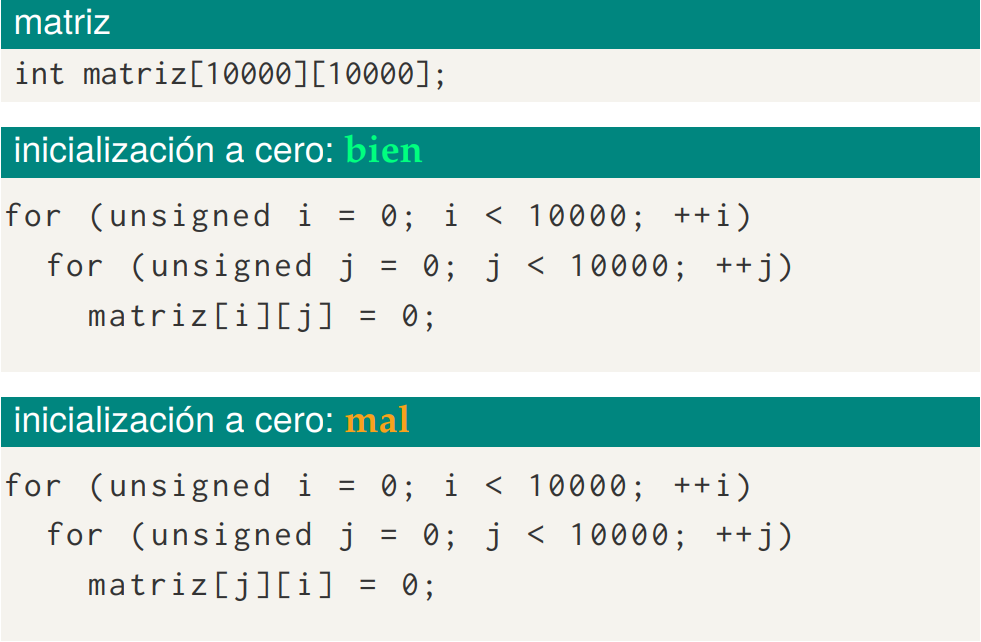
\includegraphics[scale=0.8,width=\textwidth]{gestion_memoria.png}
\end{figure}
\newpage

Para una matriz de tamaño $10000\times 10000$:
\begin{figure}[h]
\centering
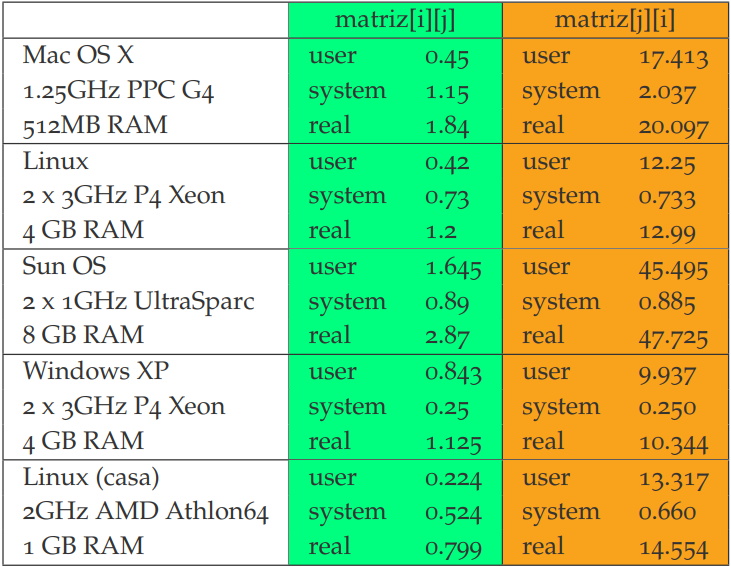
\includegraphics[scale=0.8,width=\textwidth]{time.png}
\end{figure}

La causa de este fenómeno es la forma en que C gestiona la memoria, pues C/C++ almacenan las matrices por filas. Ejemplo: $int\:\:m[4][4]$
\begin{figure}[h]
\centering
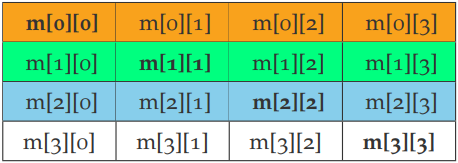
\includegraphics[scale=0.6,width=80mm]{ejemplo4x4.png}
\end{figure}

\textbf{Memoria Virtual}

Es una utilidad que permite a los programas direccionar la memoria desde un punto de vista lógico, sin importar la cantidad de memoria principal física disponible. Se concebió como método para tener múltiples trabajos de usuario residiendo en memoria principal de forma concurrente, de forma que no exista un intervalo de tiempo de espera entre la ejecución de procesos sucesivos, es decir, mientras un proceso se escribe en almacenamiento secundario y se lee el sucesor. Se introdujeron los sistemas de paginación, que permiten que los procesos se compriman en un número determinado de bloques de tamaño fijo, denominados páginas. Un programa referencia a una palabra por medio de una dirección virtual, que consiste en un número de página y un desplazamiento dentro de la página.

Todas las páginas de un proceso se mantienen en disco. Cuando un proceso está en ejecución, algunas de sus páginas se encuentran en memoria principal, y si se referencia a una página que no está en memoria principal el hardware de gestión de memoria lo detecta y permite que la página que falta se cargue (carga bajo demanda).

\subsection{Clasificación}
\subsubsection{Clasificación "práctica" de arquitecturas paralelas}
\begin{itemize}
\item Multiprocesadores de memoria compartida:
	\begin{itemize}
	\item SMT(Simultaneos Multithreading/Hyperthreading): permite a una única CPU ejecutar varios flujos de control. Esto requiere tener múltiples copias de algunos componentes hardware de la CPU, como contadores de programa y registros de archivo, mientras otras partes siguen siendo únicas como las unidades que realizan aritmética con punto flotante. Cuando un procesador tiene Hyper-Threading puede tener de 2 a 64 hebras (puede tener más, veanse procesadores de servidor), dependiendo del número de núcleos físicos del mismo.
	
	\begin{figure}[h]
	\centering
	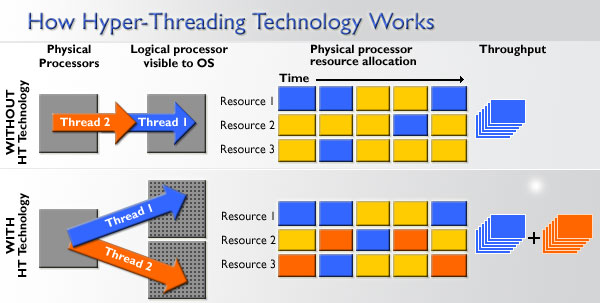
\includegraphics[scale=1,width=\textwidth]{Hyperthreading.jpg}
	\end{figure}
	
	\item SMP(Symmetric Multi-Processing): el núcleo puede ejecutar en cualquier procesador, y normalmente cada procesador realiza su propia planificación del conjunto disponible de procesos e hilos. El núcleo puede construirse como múltiples procesos o múltiples hilos, permitiéndose la ejecución de partes del núcleo en paralelo. El enfoque SMP complica el sistema operativo, ya que debe asegurar que dos procesadores no seleccionan un mismo proceso y que no se pierde ningún proceso de la cola. Se deben emplear técnicas para resolver y sincronizar el uso de los recursos. Suelen tener entre 2 y 256 procesadores.
	
	\begin{figure}[h]
	\centering
	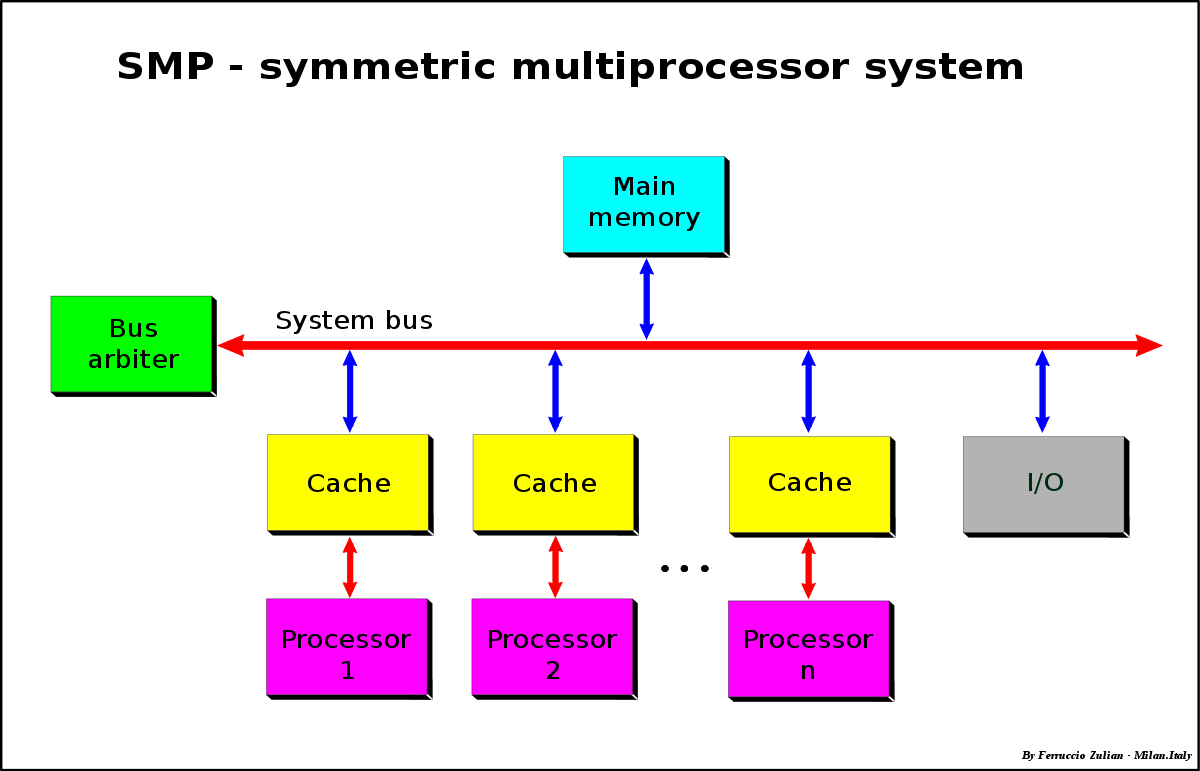
\includegraphics[scale=1,width=\textwidth]{SMP.png}
	\end{figure}
	
	\item UMA/ccNUMA (Uniforma Memory Access/Cache Coherent  UMA): Se define como la situación en la cual el acceso a cualquier RAM desde CPU toma siempre la misma cantidad de tiempo. Suele tener entre 2 y 4096 procesadores.
	
	\end{itemize}
	
\item Multiprocesadores masivamente paralelos:
	\begin{itemize}
	
	\item NUMA/ccNUMA (Non Uniform Memory Access/ Cache Coherent NUMA): A diferencia de UMA, algunas partes de la memoria pueden tomar más tiempo de acceso que otras, creando una penalización en el rendimiento. Esta penalización se puede minimizar por medio de la administración de recursos.
	
	\begin{figure}[h]
	\centering
	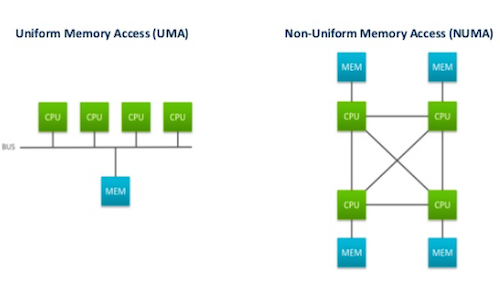
\includegraphics[scale=1,width=65mm]{umanuma.png}
	\end{figure}
	
	\item Paso de mensajes/NoRMA (No Remote Memory Access): en las arquitecturas NoRMA, el espacio de direcciones global no es único y la memoria no es globalmente accesible desde todos los procesadores. El acceso a modulos de memoria remotos es solo posible indirectamente a través del paso de mensajes por medio de la red de interconexión a otros procesadores, lo que en respuesta recibirá los datos buscados en un mensaje de respuesta.
	
	\begin{figure}[h]
	\centering
	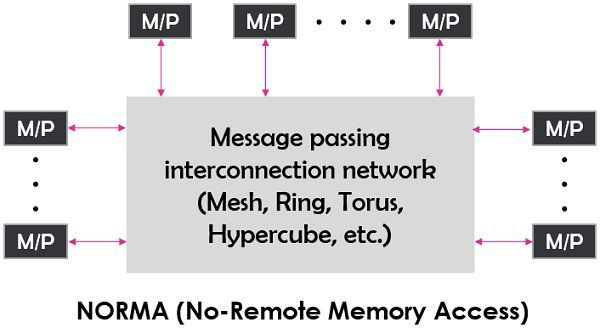
\includegraphics[scale=1,width=80mm]{NORMA.jpg}
	\end{figure}
	\end{itemize}
	
\item Cluster$\rightarrow$+10M procesadores. Al igual que los sistemas multiprocesadores, los sistemas clústes juntan múltiples CPUs para conseguir un trabajo computacional. La diferencia respecto a los sistemas multiprocesadores en que los clústers se componen de dos o más sistemas individuales unidos juntos, a los que se denominan nodos.
	\begin{itemize}
	\item GPUs
	\end{itemize}
	
	\begin{figure}[h]
	\centering
	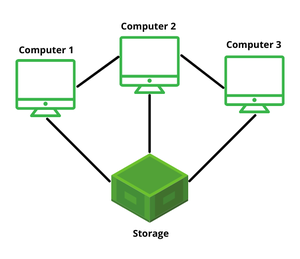
\includegraphics[scale=1,width=70mm]{cluster.png}
	\end{figure}
\end{itemize}

\subsubsection{Clasificación Arquitectura de Computadores}
\begin{itemize}
\item Sistemas monoprocesador
	\begin{itemize}
	\item Bus único
	\item Buses separados/especializados
	\end{itemize}
\item Sistemas multiprocesador
	\begin{itemize}
	\item Multiproceso simétrico (SMP)
	\item Multihebra simultánea (SMT)
	\item Multinúcleo (SMP)
	\end{itemize}
	
\item Sistemas distribuidos
\end{itemize}

\textbf{Sistema monoprocesador:} Es el modelo más simple, pues conecta todo en un bus común.
\begin{itemize}
\item Ventaja$\rightarrow$ precio.
\item Inconveniente $\rightarrow$ infrautilización de componentes por la diferencia de velocidad.
\end{itemize}

\begin{figure}[h]
\centering
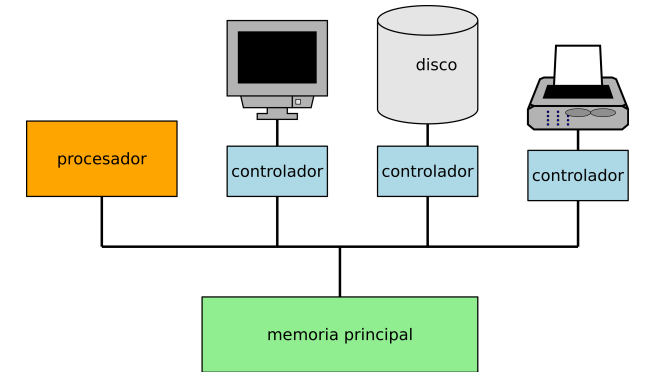
\includegraphics[scale=1,width=70mm]{monoprocesador.png}
\end{figure}

Una posible solución para la diferencia de velocidad es aislar los componentes por velocidad y conectarlos por medio de un puente

\begin{figure}[h]
\centering
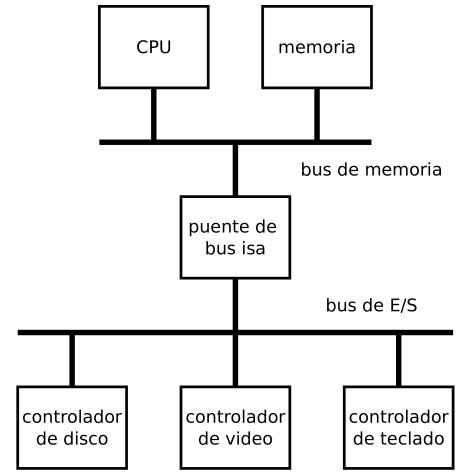
\includegraphics[scale=1,width=50mm]{solucionmonoprocesador.png}
\end{figure}
\newpage
Otra posible solución incluso mejor es separar el bus de E/S en dos buses en función de los dispositivos E/S más rápidos y más lentos, y conectar ambos buses por medio de un puente isa.

\begin{figure}[h]
\centering
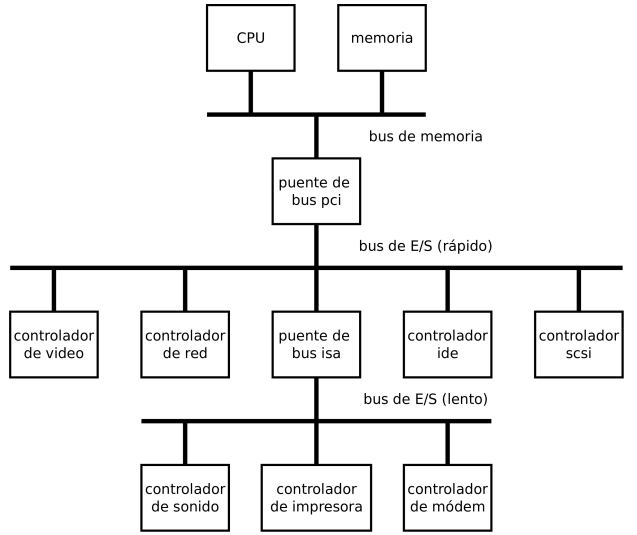
\includegraphics[scale=1,width=90mm]{sol2monoprocesador.png}
\end{figure}

\textbf{Sistema multiprocesador: multiproceso simétrico}. Lo más simple es conectar todos los elementos a un bus común.
\begin{itemize}
\item Ventaja $\rightarrow$ precio.

\item Inconveniente $\rightarrow$ se agrava la infrautilización de componentes.
\end{itemize}

\begin{figure}[h]
\centering
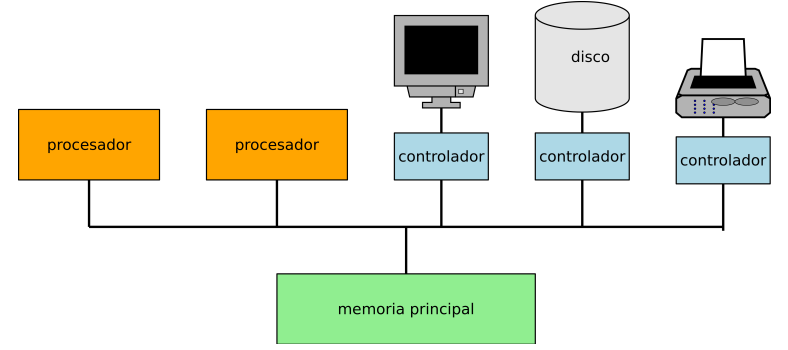
\includegraphics[scale=1,width=\textwidth]{multiprocesador.png}
\end{figure}

\newpage

\textbf{Sistemas multiprocesador: multihebra simultánea}
\begin{figure}[h]
\centering
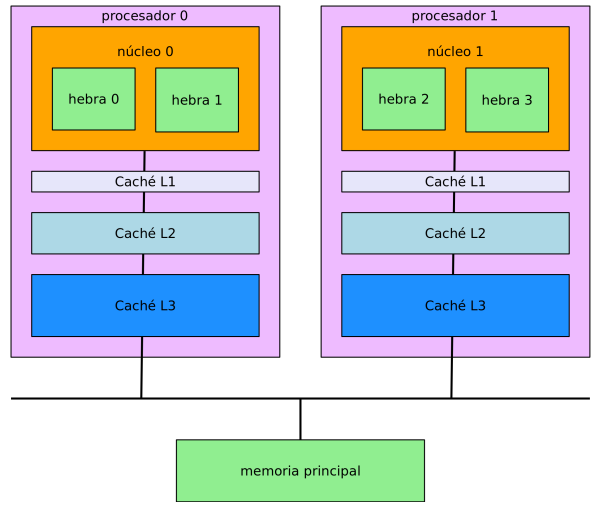
\includegraphics[scale=1,width=80mm]{multiprocesador-multihebra.png}
\end{figure}

\textbf{Sistemas multiprocesador: multiproceso simétrico}
\begin{figure}[h]
\centering
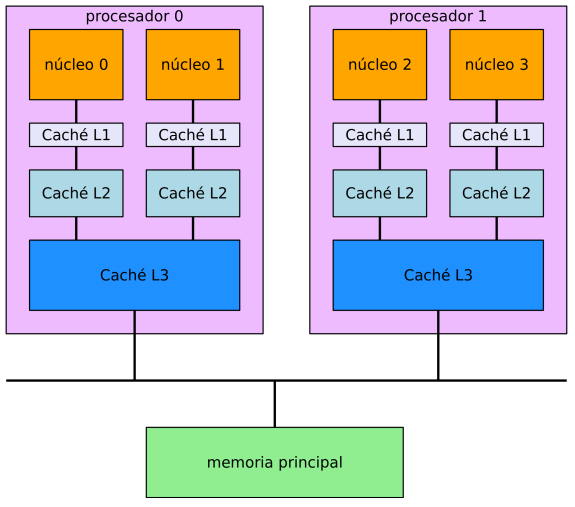
\includegraphics[scale=1,width=80mm]{multiprocesador-multihebra2.png}
\end{figure}

\newpage

\textbf{Sistemas multiprocesador actuales}
\begin{figure}[h]
\centering
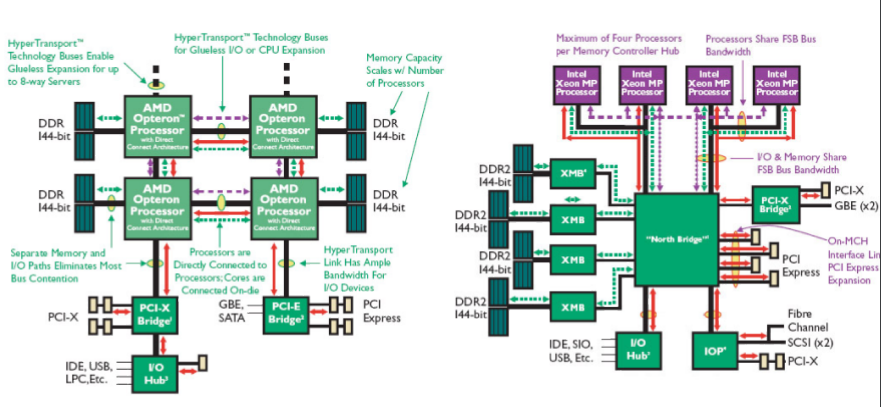
\includegraphics[scale=1,width=140mm]{multiprocesador_actual.png}
\end{figure}

\textbf{Arquitecturas de un sistema actual}
\begin{figure}[h]
\centering
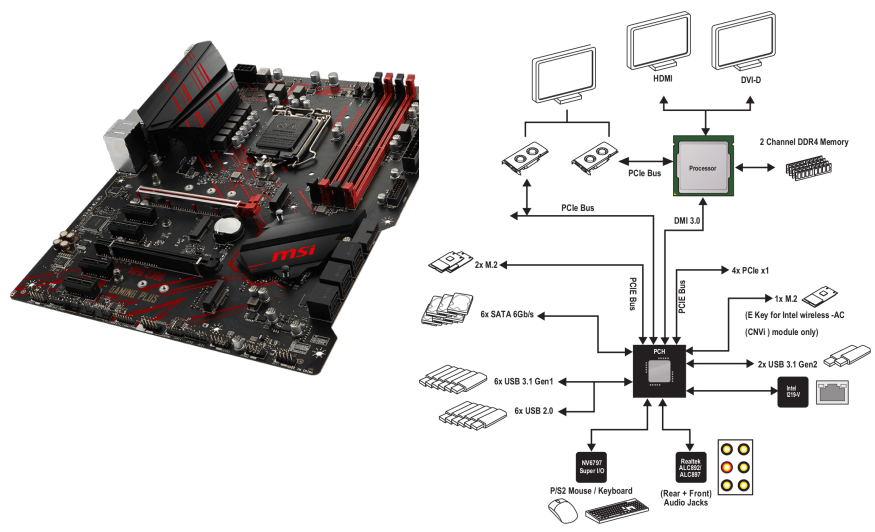
\includegraphics[scale=1,width=\textwidth]{arquitectura_actual.png}
\end{figure}

\subsubsection{Componentes}
\textbf{Componentes básicos}
\begin{itemize}
\item Procesadores
\item Jerarquía de memoria.

Surge el problema de que cuanto menor es el tiempo de acceso mayor es el coste por bit, y que cuanto mayor es la capacidad menor la velocidad de acceso. Para lidiar con este dilema surge la jerarquía de memoria. En la jerarquía de memoria según se desciende disminuye el coste por bit, aumenta la capacidad, aumenta el tiempo de acceso y se reduce la frecuencia de acceso a ese nivel de la jerarquí por parte del procesador.

\begin{figure}[h]
\centering
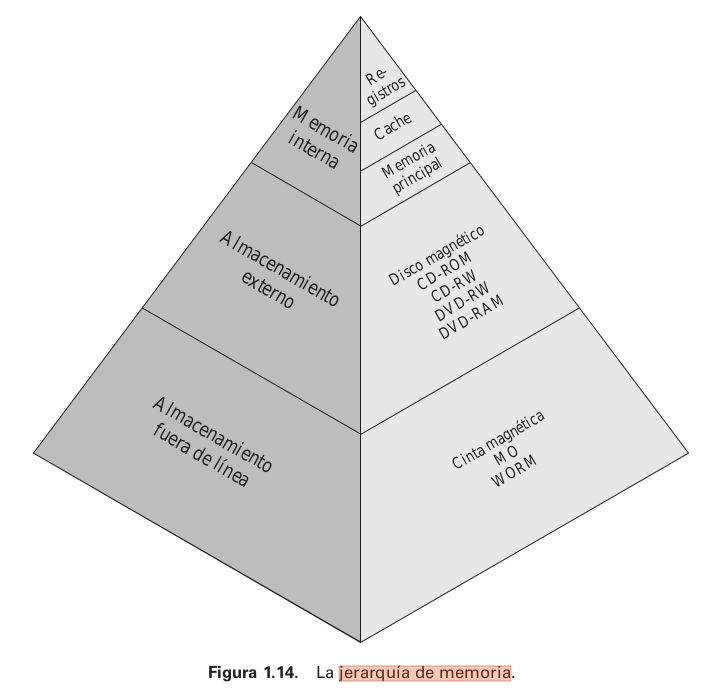
\includegraphics[scale=1,width=\textwidth]{jerarquiamemoria.png}
\end{figure}


\item Buses de interconexión: AGP, Hypertransport, IDE, IEEE 1394, ISA, M.2, PCI, PCIe, SATA, SCSI, USB, ...
\item Entrada/Salida: controladores, canales de DMA, procesadores de E/S,...
\item Periféricos: altavoz, disco, impresora, micrófono, monitor, ratón, teclado, ...
\end{itemize}

\subsubsection{Procesador}
\textbf{Interfaz del procesador}
\begin{itemize}
\item Conjunto de instrucciones
	\begin{itemize}
	\item transferencia: \begin{verbatim}
	in, mov, out,...
	\end{verbatim}
	
	\item modificación: \begin{verbatim}
	add, and, div, mul, or, sub,...
	\end{verbatim}
	
	\item control: \begin{verbatim}
	cli, sti,...
	\end{verbatim}
	
	\href{http://jegerlehner.ch/intel/IntelCodeTable_es.pdf}{Chuleta instrucciones 8086}
	\end{itemize}

\item Registros generales y especiales

\item Al menos dos modos de ejecución con diferentes privilegios:
	\begin{itemize}
	\item privilegiado: acceso completo
	\item no privilegiado: acceso limitado $\Rightarrow$ excepción
	\end{itemize}
	
\begin{figure}[h]
\centering
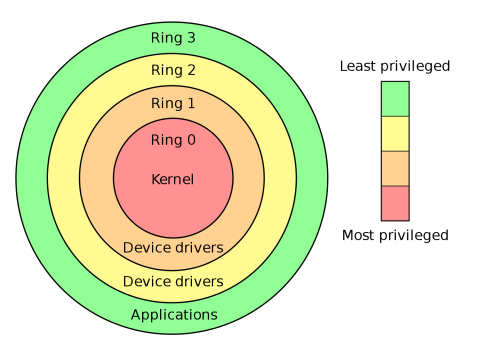
\includegraphics[scale=1,width=\textwidth]{privilegios.png}
\end{figure}
\end{itemize}

\href{https://upload.wikimedia.org/wikipedia/commons/4/41/Table_of_x86_Registers.png}{Registros del procesador: familia x86-64} \\

En el modo núcleo (modo privilegiado, modo kernel, ...) se pueden ejecutar instrucciones privilegiadas y se puede accesder a áreas de memoria protegidas. Sóla mente el núcleo o kernel del sistema operativo puede ejecutar instrucciones en modo privilegiado. Algunos ejemplos de instrucciones privilegiadas son:

\begin{itemize}
\item Acceso a los dispositivos de E/S: consultar el estado de los dispositivos de E/S, llevar a cabo DMA (Direct Memory Access), atrapar interrupciones.

\item Manipular la unidad de gestión de memoria (MMU): manipualar las tablas de segmento y páginas, cargar y vaciar el búfer de traducción anticipada (TLB)

\item Configurar varios modos de funcionamiento: nivel de prioridad de interrupciones, alterar el vector de interrupción.

\item Utilizar la instrucción $halt$ para activar el modo de ahorro de energía. Esta instrucción detiene abruptamente la CPU hasta que la siguiente interrupción externa ha sido tratada. También es común que se ejecute cuando no hay trabajo inmediato que ejecutar, de forma que se pone al procesador en un estado ocioso.
\end{itemize}

El procesador comprueba el nivel de privilegio en la ejecución de cada instrucción. Los posibles cambios de privilegio son:

\begin{itemize}
\item Usuario $\Rightarrow$ Núcleo: ganar privilegios
	\begin{itemize}
	\item Al arrancar.
	\item Llamada al sistema.
	\item Interrupción hardware.
	\item Excepción.
	\end{itemize}
	
\item Núcleo $\Rightarrow$ Usuario: perder privilegios
	\begin{itemize}
	\item El sistema operativo prepara el entorno necesario para que la aplicación comience su ejecución.
	
	\item El sistema operativo termina alguna de sus actividades y devuelve el control a la aplicación.
	\end{itemize}
\end{itemize}

\textbf{Ciclo de instrucción:} se denomina ciclo de instrucción al procesamiento requerido por una única instrucción. El ciclo de instrucción básco es:

\begin{figure}[h]
\centering
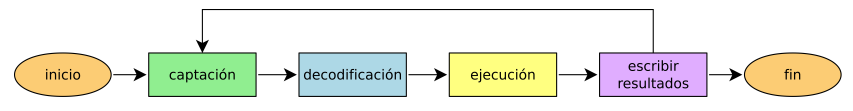
\includegraphics[scale=1,width=\textwidth]{ciclo_instruccion.png}
\end{figure}

\begin{itemize}
\item El procesador capta una instrucción desde memoria.

\item La instrucción debe ser decodificada para averiguar su tipo.

\item Conocido el tipo puede ser necesario la captación de nuevos operandos.

\item Se ejecuta la instrucción.

\item Se almacenan los resultados de la ejecución.

\item El proceso se repite instrucción a instrucción hasta que el programa termina.
\end{itemize}

\textbf{Tendencias en el diseño de procesadores}
\begin{itemize}
\item CISC (Complex Instruction Set Computing)$\Rightarrow$ RISC (Reduced Instruction Set Computing) $\Rightarrow$ VLIW (Very Long Instruction Word).

\textbf{CISC}: Es un tipo de diseño de microprocesador. Este contiene un conjunto de instrucciones muy grande que van desde instrucciones muy simples a instrucciones muy especializadas. Se introducen instrucciones que en un diseño RISC se requieren de varias instrucciones, reduciendo así el número de instrucciones de los programas, pero al ser instrucciones más complejas acaban requiriendo más ciclos de reloj para su ejecución.\\

\textbf{RISC}: Como su nombre dice se trata de un diseño de microprocesador. Este diseño contiene instrucciones muy simples y con la combinación de ellas se puede obtener cualquier programa. Si bien su ejecución es rápida, pues son instrucciones muy simples, su tamaño en memoria puede llegar a ser muy grande, pues la ejecución de un programa simple puede requerir de muchas instrucciones RISC.

\textbf{VLIW}: se trata de un procesador segmentado que puede terminar más de una operación por ciclo en el que el compilador es el principal responsable de agrupar operaciones que pueden procesarse en paralelo para definir instrucciones que, de esta forma, se codifican a través de las denominadas palabras de instrucción larga (LIW) o muy larga (VLIW)

\item Ejecución concurrente sobre procesadores: intento de explotación del paralelismo entre instrucciones (ILP). ILP es una mediad de cuántas operaciones pueden ejecutarse simultáneamente sin afectar al resultado.
\end{itemize}

\textbf{Técnicas de explotación de ILP}
\begin{itemize}
\item \textbf{Segmentación de cauce:} la ejecución de múltiples instrucciones puede solaparse total o parcialmente. 

\begin{figure}[h]
\centering
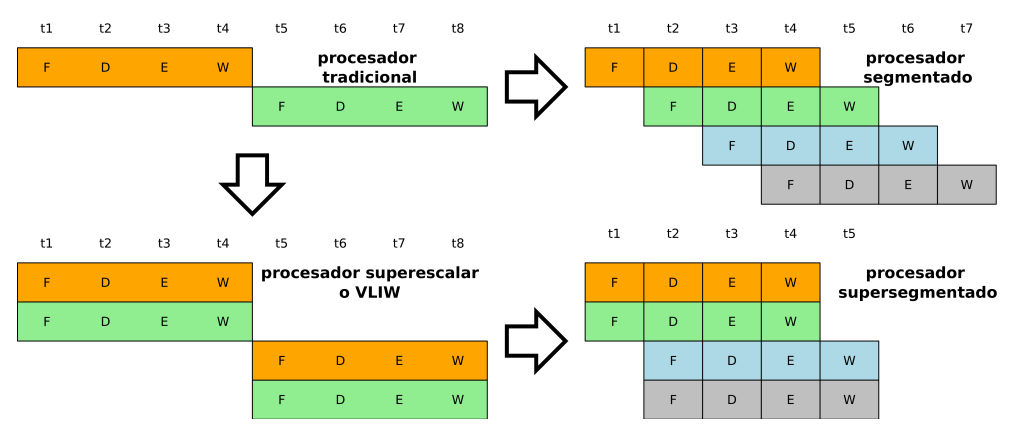
\includegraphics[scale=1,width=\textwidth]{segmentacion.png}
\end{figure}

\item \textbf{Ejecución superescalar:} múltiples unidades de ejecución se utilizan para ejecutar múltiples instrucciones en paralelo. Un procesador superescalar es un procesador segmentado que puede finalizar más de una instrucción por ciclo y que posee recursos hardware para extraer el paralelismo entre instrucciones. Para aprovechar al máximo el procesamiento de instrucciones en paralelo que proporcionan las distintas estapas, el procesador incluye una serie de elementos como ventanas de instruccioens o estaciones de buffers, buffers de renombramiento, buffers de reordenamiento, etc.

\item \textbf{Computación con instrucciones explícitamente paralelas (EPIC):} uso del compilador en lugar de complejos circuitos para identificar y explotar el ILP. La intención era permiter un escalado simple del rendimiento sin disparar las frecuencias del reloj. Tiene su base en VLIW.

\item \textbf{Ejecución fuera de orden:} ejecución de instrucciones en cualquier orden que no viole las dependencias entre instrucciones. El orden de ejecución depende de la disponibilidad de los datos de entrada y las unidades de ejecución, no del orden original del programa.

\item \textbf{Renombrado de registros:} técnica para evitar la innecesaria serialización de instrucciones por la reutilización de registros. Puede ser aplicado por el propio compilador al asignar los registros de la arquitectura, pero también puede implementarse en hardware. Esto es lo usual en procesadores superescalares, donde se incluyen estructuras de buffers con una serie de campos específicos (por ejemplo, buffers de renombramiento).

\item \textbf{Ejecución especulativa:} permitir la ejecución de instrucciones completas, o partes, antes de conocer con seguridad si su ejecución debe tener lugar. De esta forma se previene el retraso que habría, de tener que hacer el procesamiento después de saber que es necesario. Si resulta que el procesamiento no era necesario, los cambios realizados se revierten y los resultados se ignoran.

\item \textbf{Predicción de salto:} se utiliza para evitar quedar parado antes de que se resuelvan las dependencias de control. Se utiliza en conjuntción con la ejecución especulativa. Se basa en determinar la alternativa más probable, y continuar el procesamiento, tras las instrucción de salto, con la secuencia de instrucciones que corresponde a dicha opción más probable. Cuando la condición de salto se evalúa, se comprueba si la predicción que se había hecho era correcta o no. Si no lo era habrá que retomar el procesamiento a partir de la primera instrucción de la alternativa que no se tomó, es decir, de la menos probable.

\begin{figure}[h]
\centering
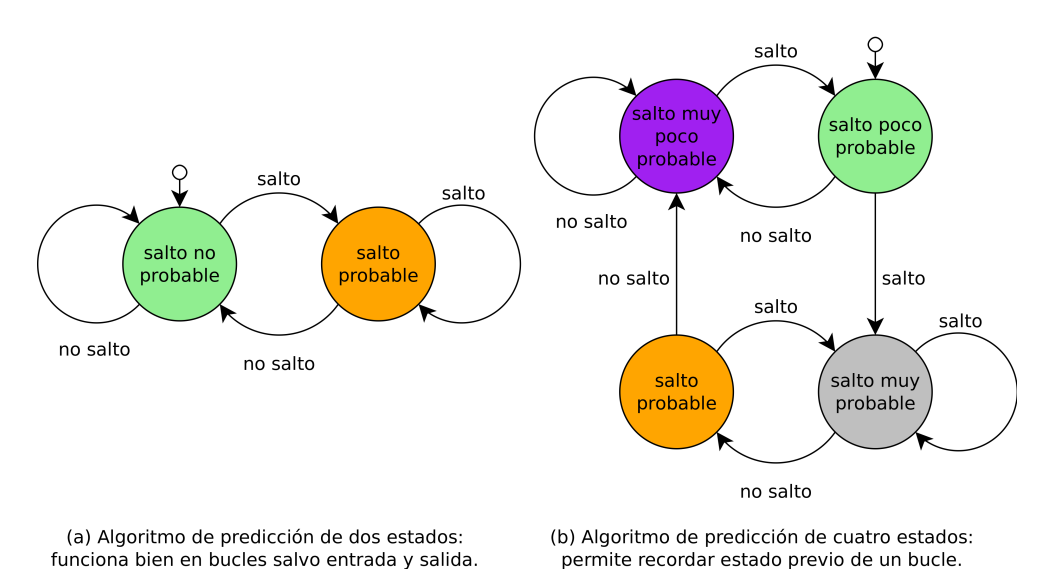
\includegraphics[scale=1,width=\textwidth]{predicionsalto.png}
\end{figure}

\item \textbf{Multihebra simultánea (SMT):} técnica que permite la ejecución de múltiples hebras de ejecución para aprovechar mejor las unidades funcionales de los procesadores superescalares.
\end{itemize}

\subsubsection{Memoria}

\textbf{Jerarquía de memoria:} Se requiere de jerarquía de memoria entre otras cosas por la gran diferencia de velocidad entre procesador y memoria. La jerarquía de memoria puede aliviar este problema gracias a \textbf{los principios de localidad} y a la \textbf{regla 90/10}:
\begin{itemize}
\item Localidad \textbf{espacial:} la información a la que se accede suelen estar próxima a la que ha sido accedida con anterioridad.

\item Localidad \textbf{temporal:} la información a la que se accede una vez suele volver a ser utilizada.

\item Regla 90/10: el 10\% del código realiza el 90\% del trabajo.
\end{itemize}

\textbf{Tipos de memoria RAM}:
\begin{figure}[h]
\centering
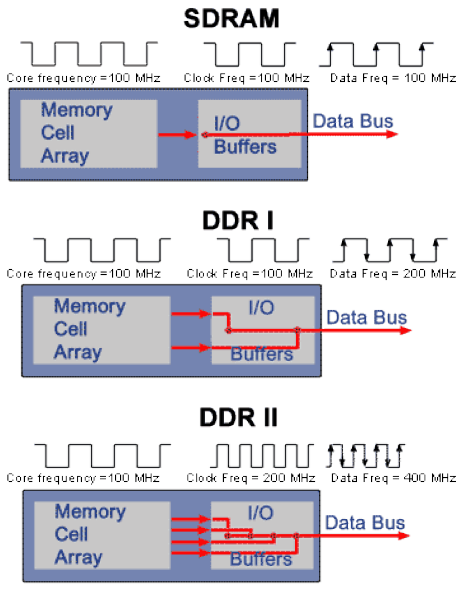
\includegraphics[scale=1,width=80mm]{tiposram.png}
\end{figure}
\begin{itemize}
\item SRAM (Statica random-access memory): Es un tipo de memoria que utiliza circuitería flip-flop para almacenar cada bit. La diferencia con una DRAM es que la segunda debe de refrescarse periódicamente. La SRAM es más rápida y más cara que la DRAM. Se utiliza típicamente para la caché y los registros internos de la CPU mientras que la DRAM se utiliza para la memoria principal.

\item DDR SDRAM I (Double Data Rate Synchronous RAM): Entre otras cosas las memorias DDR como su nombre indica tienen dos ciclos de reloj, es decir se hace un envío de información cuando el reloj sube y otro cuando el reloj baja. Con esto hace que una memoria DDR con una frecuencia de reloj x duplique el ancho de banda de una SDR SDRAM con igual frecuencia de reloj. Este tipo de memoria se ha visto superada por las versiones 2, 3, 4 y 5 de la misma. Ninguno de sus sucesores tienen compatibilidad ni con su predecesor ni con su sucesor, lo que quiere decir que una RAM DDR1 SDRAM no es compatible con DDR2, DDR3, .... 
\item DDRAM II
\end{itemize}

\textbf{Cantidad de memoria en registros}
\begin{itemize}
\item Tipos de registros:

\item RISC:
	\begin{itemize}
	\item 32 de propósito general (32 ó 64 bits)
	\item 32 de punto flotante (64 bits IEEE 754)
	\item multimedia (64,...,256 bits)
	\end{itemize}

\item CISC: 
	\begin{itemize}
	\item IA32: 8 de propósito general, 8 de punto flotante, 8 multimeida.
	\item IA64: 128 de propósito general, 128 de punto flotante.
	\end{itemize}

\item Algunos procesadores tienen varios conjuntos de estos registros (ventanas de registros)
\end{itemize}

\textbf{Análisis de una jerarquía de dos niveles}
\begin{equation*}
\overline{T}_{acceso}=(1-T_{fallos})\times T_{cache}+T_{fallos}\times(T_{cache}+T_{ram})
\end{equation*}

\textbf{Parámetros de diseño de memorias caché}
\begin{itemize}
\item Tamaño:
	\begin{itemize}
	\item L1:8,...,256KB
	\item L2:1,...,16MB
	\item L3:4,...,128MB
	\end{itemize}
	
\item Tamaño de bloque: 32,...,128B

\item Tiempo de acceso: 1,...,10ns

\item Política de búsqueda:
	\begin{itemize}
	\item bajo demanda
	\item anticipativas
	\end{itemize}

\item Política de colocación:
	\begin{itemize}
	\item correspondencia directa: el bloque $B_j$ de memoria principal se puede ubicar sólo en el marco de bloque que cumple la siguiente relación $i=j\mod{m}$, donde $m$ es el número total de líneas que tiene la cache.
	
	\item asociativa por conjuntos: En la corresponcencia asociativa por conjuntos las líneas de memoria caché se agrupan en $v=2^d$ conjunto con $k$ líneas/conjuto o vías. Se cumple que el número total de marcos de bloque que tiene la caché $m=v*k$. Un bloque $B_j$ de memoria principal se puede ubicar sólo en el conjunto $C_i$ de memoria caché que cumple la siguiente relación $i=j\mod{v}$.
	
	\item completamente asociativa: la caché se organiza en un único conjunto de caché con varias líneas de caché. Un bloque de memoria puede ocupar cualquiera de las lineas de caché. La organización de la caché se puede enmarcar como una matriz de filas (1*m).
	\end{itemize}
	
\item Política de reemplazo:
	\begin{itemize}
	\item LRU
	\item FIFO
	\item aleatoria
	\end{itemize}

\item Política de actualización:
	\begin{itemize}
	\item escritura directa
	\item post-escritura
	\end{itemize}

\item Otras características importantes:
	\begin{itemize}
	\item caché de víctimas
	\item inclusiva/exclusiva
	\item unificada/separada
	\end{itemize}
\end{itemize}

\textbf{Políticas de colocación: correspondencia directa}
\begin{figure}[h]
\centering
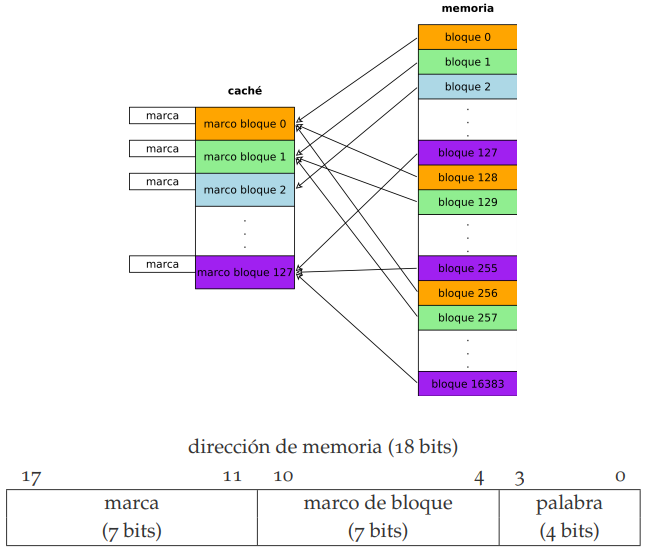
\includegraphics[scale=1,width=85mm]{correspondenciadirecta.png}
\end{figure}
\newpage

\textbf{Políticas de colocación: correspondencia totalmente asociativa}
\begin{figure}[h]
\centering
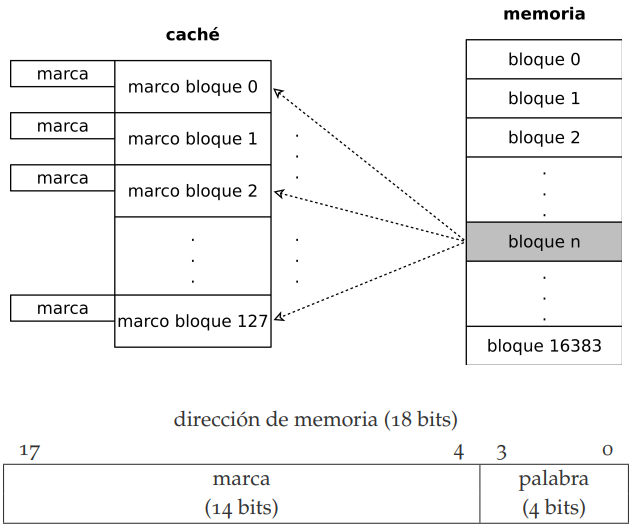
\includegraphics[scale=1,width=85mm]{totalmenteasociativa.png}
\end{figure}

\newpage

\textbf{Políticas de colocación: correspondencia asociativa por conjuntos (2 M/C)}
\begin{figure}[h]
\centering
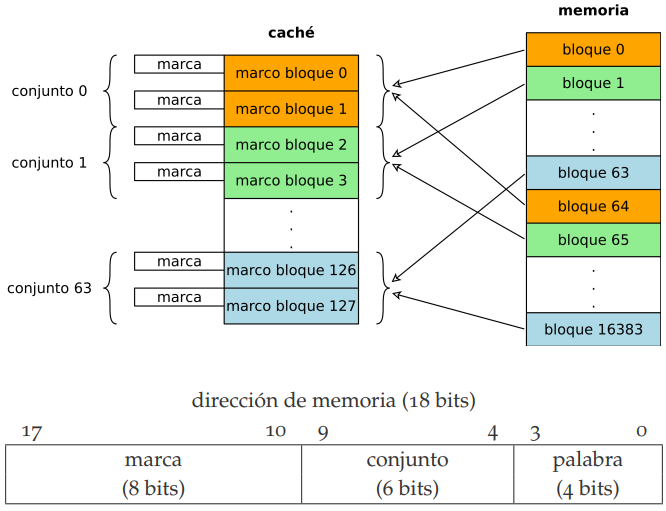
\includegraphics[scale=1,width=85mm]{porconjuntos.png}
\end{figure}

\textbf{Protección de memoria.}

El sistema operativo debe proteger a los programas entre sí y a él mismo de programas maliciosos o erróneos. Este problema se soluciona utilizando los llamados espacios de direcciones (AS, Address Space). El espacio de direcciones de un computador corresponde al rango de direcciones disponible para un programa de computador.

El procesador dispone de recursos para establecer límites al espacio de direcciones de memoria accesibles por los programas: memoria virtual.

\begin{figure}
\centering
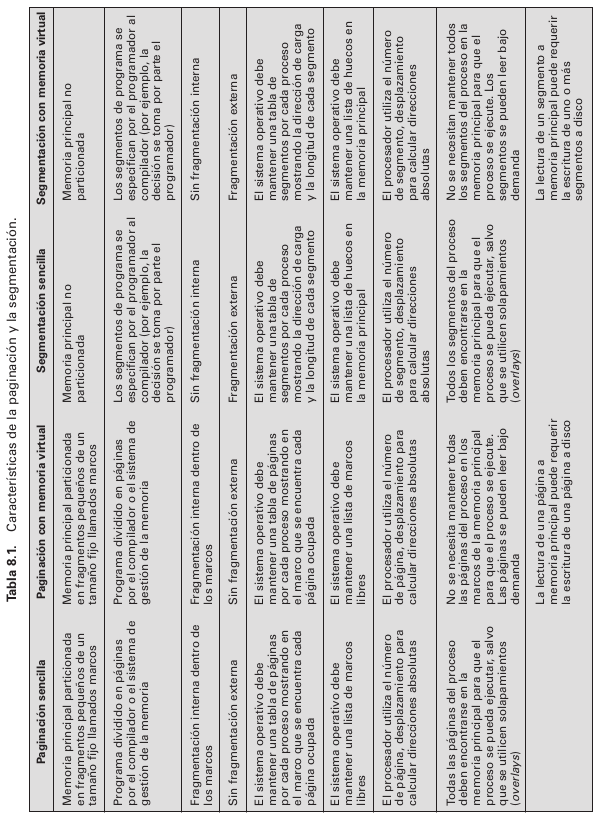
\includegraphics[scale=1,width=\textwidth]{memvirtual.png}
\end{figure}
\newpage

Hay varias implementaciones:

\begin{itemize}
\item Segmentaciones: tamaño variable y arbitrario.
	\begin{itemize}
	\item registro base: principio del espacio de direcciones.
	\item registro límite: tamaño del espacio de direcciones.
	\end{itemize}

\item Paginación: tamaño variable en múltiplos de página.
	\begin{itemize}
	\item tablas de páginas: lista de páginas de un proceso.
	\end{itemize}
\end{itemize} 

La mayoría de los SO asocian un espacio de direcciones diferente para cada proceso (salvo SASOS, Single Adrress Space Operating System):
\begin{itemize}
\item Ventaja $\Rightarrow$ protección automática.

\item Inconveniente $\Rightarrow$ dificulta la compartición
\end{itemize}

Las partes de un espacio de direcciones pueden colocarse en cualquier parte de la memoria física. Algunos espacios de direcciones deben ocupar lugares específicos de la memoria física, ej: dispositivos de E/S.

El procesador debe tener una unidad de gestión de memoria (MMU, Memory Management Unit) extremadamente eficiente porque la traducción entre direcciones virtual-física puede realizarse más de una vez por instrucción. Se requiere una traducción por cada acceso a memoria.\\

\textbf{Traducción de dirección virutal a dirección física}
\begin{enumerate}
\item La ejecución de una instrucción puede requerir varias traducciones, por ejemplo:
	\begin{itemize}
	\item Captacińo de la instrucción.
	
	\item Captación del dato.
	
	\item Escritura del resultado.
	\end{itemize}
	
\item Cada traducción puede requerir varios accesos a memoria:
	\begin{itemize}
	\item Segmentación + paginación.
	
	\item Tablas de página multinivel.
	\end{itemize}
	
\item Se necesita una tabla de traducción por cada espacio de direcciones.

\item Dependerá del tamaño de las direcciones virtuales y físicas, pero habrán al menos tantas entradas como páginas tenga el proceso.
\end{enumerate}

\begin{figure}[h]
\centering
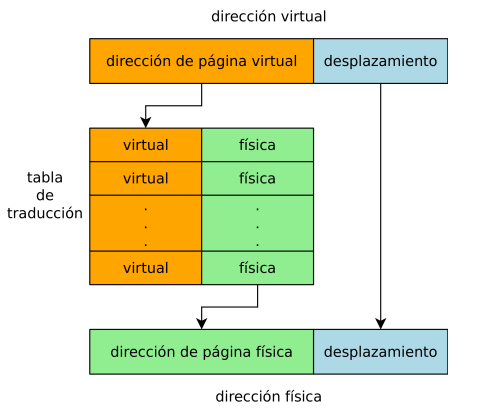
\includegraphics[scale=1,width=80mm]{traduccion.png}
\end{figure}
\newpage

\textbf{Fucnionamiento de la segmentación (x86)}
\begin{figure}[h]
\centering
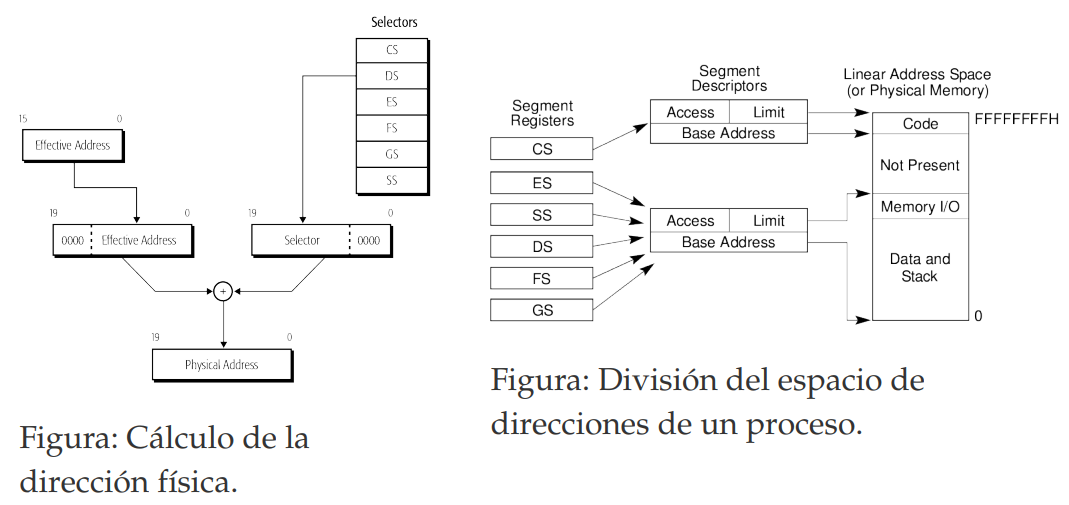
\includegraphics[scale=1,width=\textwidth]{segmentacionx86.png}
\end{figure}
\newpage

\textbf{Segmentación + paginación (x86\_64)}
\begin{figure}[h]
\centering
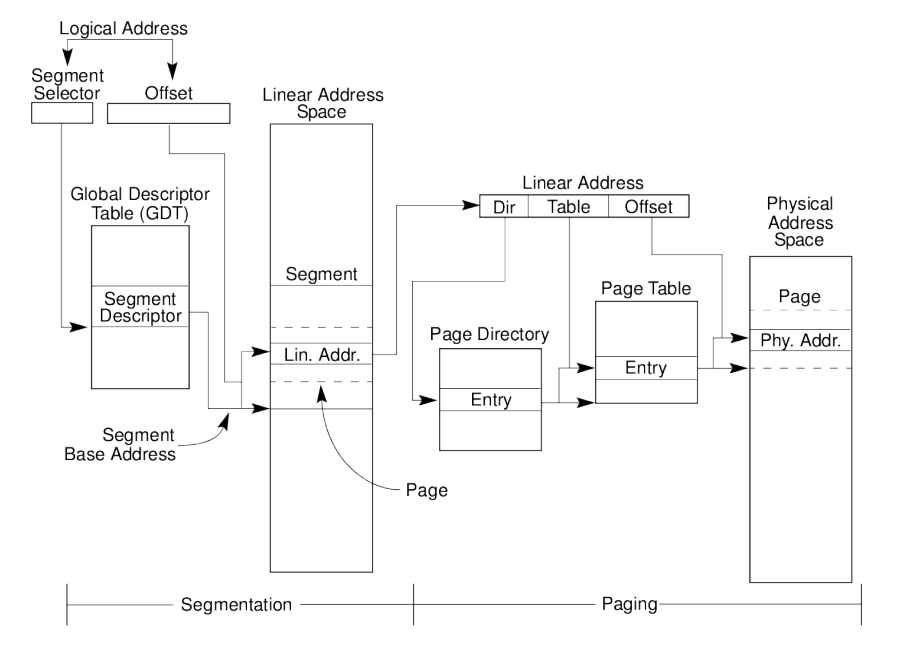
\includegraphics[scale=1,width=90mm]{segmentacionpaginacion.png}
\end{figure}

\textbf{Tabla de páginas multinivel (x86\_64)}
\begin{figure}[h]
\centering
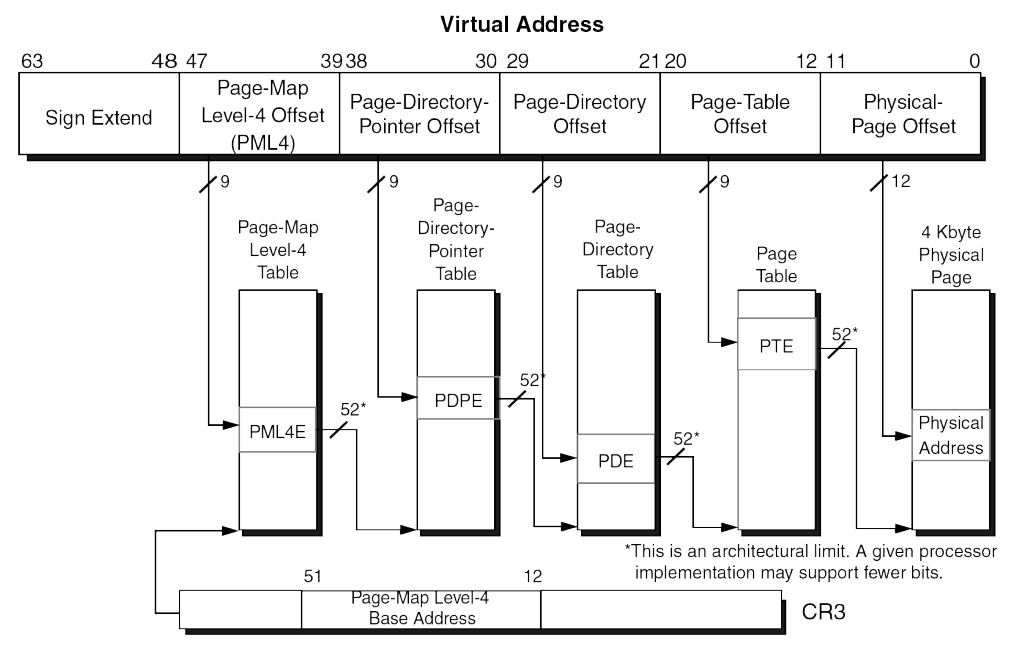
\includegraphics[scale=1,width=85mm]{tabla_multinivel.png}
\end{figure}

\newpage

\textbf{Estructura habitual tabla de páginas}
\begin{figure}[h]
\centering
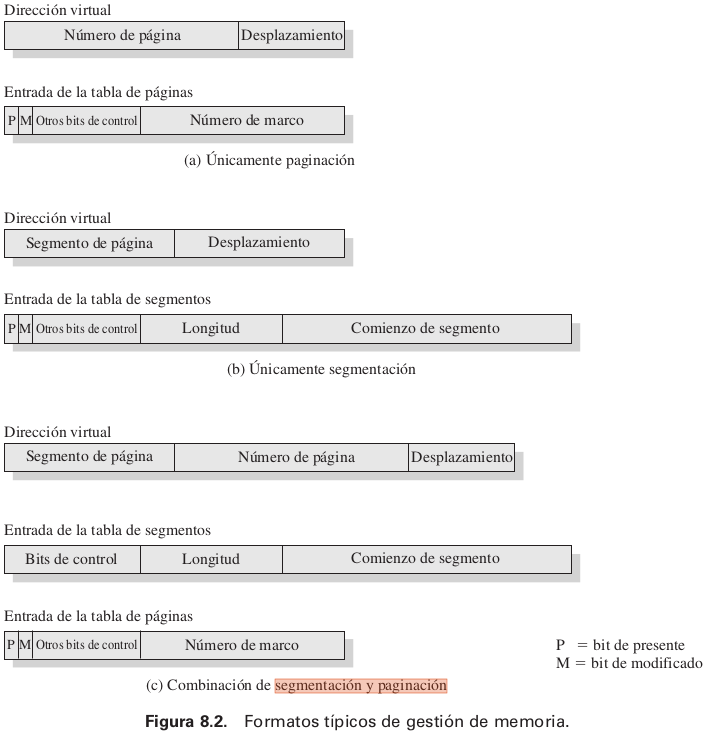
\includegraphics[scale=1,width=\textwidth]{estructuratabla.png}
\end{figure}

\subsubsection{Interacción}
\textbf{Buffer de traducción anticipada (TLB)}

Traducir direcciones por software es muy lento, mientras que mediante hardware puede hacerse más rápido y además podemos añadir una caché de traducciones (TLB). En principio, toda referencia a la memoria virtual puede causar dos accesos a memoria física, uno para buscar la entrada en la tabla de página apropiada y otra para buscar los datos solicitados. De esa forma, el esquema de memoria virtual básico causaría el efecto de duplicar el tiempo de acceso a la memoria. Para solventar este problema, la mayoría de esquemas de la memoria virtual utilizan una \textit{cache} especial de alta velocidad para las entradas de la tabla de páginas, habitualmente denominada buffer de traducción anticipada. TLB:
\begin{itemize}
\item Conenido: pares de direcciones virtual/física.

\item Implementado mediante memorias asociativas.

\item Tamaño típico: de 32 a 128 entradas.
\end{itemize}

Hay dos tipos fundamentales:
\begin{itemize}
\item Etiquetadas: añaden una marca del espacio de direcciones al que pertenece.

\item No etiquetadas: no poseen la capacidad anterior, la mayoría.
\end{itemize}

Funcionamiento:
\begin{itemize}
\item Si se encuentra la dirección en el TLB se devuelve su traducción.

\item Si no se encuentra es necesario calcular la traducción.
	\begin{itemize}
	\item Hardware: se devuelve la traducción correcta (x86).
	
	\item Software: más lento pero más flexible (PowerPC).
	\end{itemize}

\item Es fundamental conocer la interacción TLB/caché.
\end{itemize}

\begin{figure}[h]
\centering
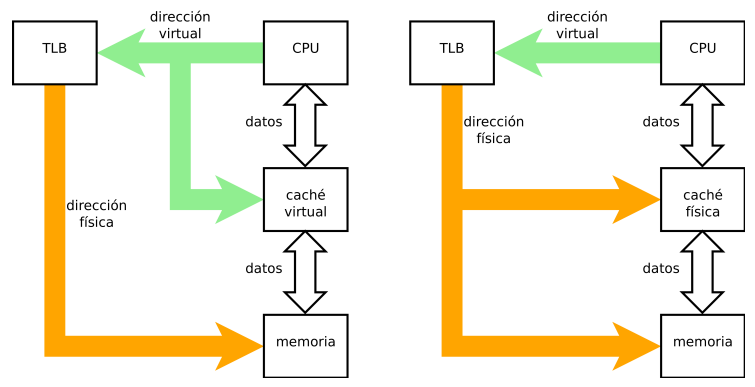
\includegraphics[scale=1,width=\textwidth]{direccionamientocache.png}
\end{figure}

El proceso que sigue generalmente es el siguiente:
\begin{enumerate}
\item Dada una dirección virtual, el procesador primero examina la TLB.

\item Si la entrada de la tabla de páginas solicitada está presente (acierto en la TLB), entonces se recupera el número de marco y se construye la dirección real.

\item Si la entrada de la tabla de páginas no se encuentra (fallo en la TLB), el procesador utiliza el número de página para indexar la tabla de páginas del proceso y examinar la correspondiente entrada de la tabla de páginas.
	
	\begin{enumerate}
	\item Si el bit de presente está puesto a 1, entonces la página se encuentra en memoria principal, y el procesador puede recuperar el número de marco desde la entrada de la tabla de páginas para construir la dirección real. El procesador también autorizará la TLB para incluir este nueva entrada de tabla de páginas.
	
	\item Si el bit presente no está puesto a 1, entonces la página solicitada no se encuentra en memoria principal y se produce un fallo de acceso memoria, llamado \textbf{fallo de página}.
	\end{enumerate}
\end{enumerate}

\begin{figure}[h]
\centering
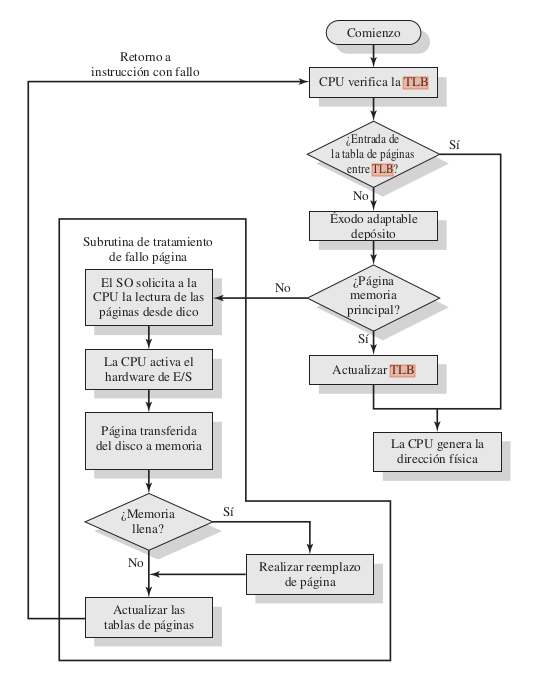
\includegraphics[scale=1,width=90mm]{TLB.png}
\end{figure}

\newpage

\textbf{Esquemas de direccionamiento de caché}
\begin{figure}[h]
\centering
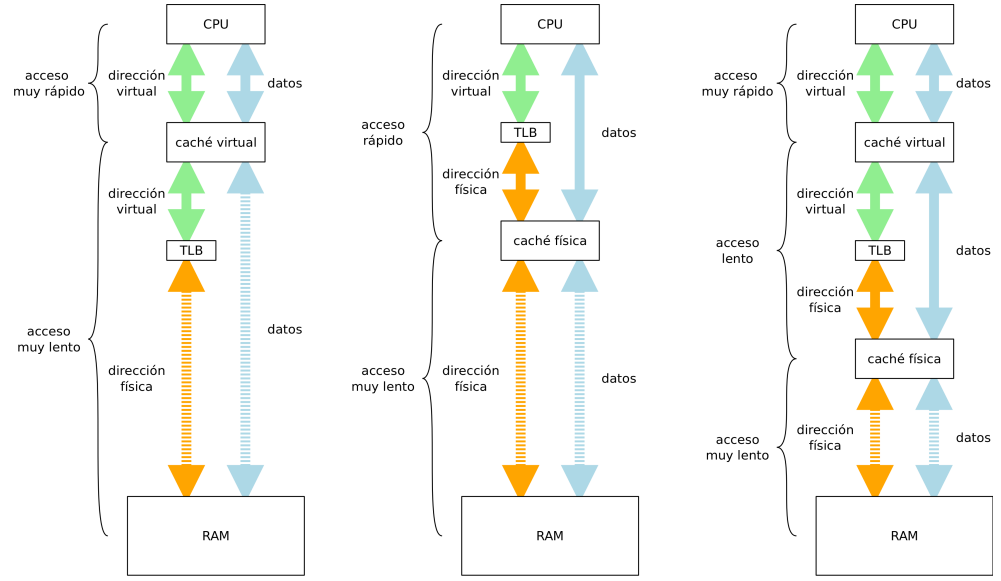
\includegraphics[scale=1,width=\textwidth]{esquemacache.png}
\end{figure}

\textbf{Control de Entrada/Salida}

El sistema operativo inicia una operación E/S:
\begin{itemize}
\item Instrucciones especiales: \textbf{in}/\textbf{out} (x86)

\item E/S en memoria: \textbf{mov} (x86)
	\begin{itemize}
	\item Acceso al hardware como direcciones de memoria.
	\item Requiere de una MMU capaz de traducir el bus de E/S.
	\end{itemize}
\end{itemize}

Por otro lado es SO puede averiguar cuando una orden E/S finaliza de las siguientes formas:
\begin{itemize}
\item Sondeo: leer el puerto de estado hasta encontrar el valor adecuado. La CPU continuamente rueba todos y cada uno de los dispositivos conectados a él para detectar si algún dispositivo necesita atención de la CPU. Algoritmo de sondeo:
	\begin{enumerate}
	\item Cuando un dispositivo tiene algún comando para ser ejecutado por la CPU, comprueba continuamente el bit de ocupado de la CPU hasta que se borra (0).
	
	\item Cuando se borra el bit de ocupado, el dispositivo establece el bit de escritura en su registro de comando y escribe un byte en el registro de salida de datos.
	
	\item Ahora el dispositivo establece (1) el bit de comando listo.
	
	\item Cuando la CPU verifica el bit de comando listo y lo encuentra establecido (1), establece (1) su bit de ocupado.
	
	\item Luego, la CPU lee el registro de comando del dispositivo y ejecuta el comando del dispositivo.
	
	\item Después de la ejecución del comando, la CPU borra (0) el bit de comando listo, el bit de error del dispositivo para indicar la ejecución exitosa del comando del dispositivo y además borra (0) su bit de ocupado para indicar que la CPU está libre para ejecutar el comando de algún otro dispositivo.
	\end{enumerate}	 

\item Interrupción: existe una línea física mediante la cual se avisa del fin de la operación y se cede el control al SO. Procesamiento de interrupciones:
	\begin{enumerate}
	\item El dispositivo genera una señal de interrupción hacia el procesador.
	
	\item El procesador termina la ejecución de la instrucción actual antes de responder a la interrupción.
	
	\item El procesador comprueba si hay petición de interrupción pendiente, determina que hay una y manda y una señal de reconocimiento al dispositivo que produjo la interrupción. Este reconocimiento permite que el dispositivo elimine su señal de interrupción.
	
	\item En ese momento, el procesador necesita prepararse para transferir el control a la rutina de interrupción. Para comenzar, necesita salvar la información requerida para reanudar el programa actual en el momento de la interrupción. La información mínima requerida es la palabra de estado del programa (PSW) y la posición de la siguiente instrucción que se va a ejecutar, que está contenida en el contador de programa. Esta información se peude apilar en la pila de control de sistema.
	
	\item A continuación, el procesador carga del contador del programa con la posición del punto de entrada de la rutina de interrupción que responderá a esta interrupción. Dependiendo de la arquitectura de computador y del diseño del sistema operativo, puede haber un único programa, uno por cada tipo de interrupción o uno por cada dispositivo y tipo de interrupción. Si hay más de una rutina de manejo de interrupción, el procesador debe determinar cuál invocar. Esta información puede estar incluida en la señal de interrupción original o el procesador puede tener que realizar una petición al dispositivo que generó la interrupción para obtener una respuesta que contiene la información requerida.
	
	\item En este momento, el contador del programa y la PSW vinculados con el programa interrumpido se han almacenado en la pila del sistema. Sin embargo, hay otra información que se considera parte del estado del programa en ejecución. En concreto, se necesita salvar el contenido de los registros del procesador, puesto que estos registros los podría utilizar el manejador de interrupciones. Por tanto, se deben salvar todos estos valores, así como cualquier otra información de estado. Generalmente, el manejador de interrupción comenzará salvando el contenido de todos los registros en pila. 
	
	\item El manejador de interrupción puede en este momento comenzar a procesar la interrupción. Esto incluirá un examen de la información de estado relacionada con la operación de E/S o con otro evento distinto que haya causado la interrupción. Asimismo, puede implicar el envío de mandtos adicionales o reconocimientos al dispositivo de E/S.
	
	\item Cuando se completa el procesamiento de la interrupción, se recuperarn los valores de los registros salvados en la pila y se restituyen los registros.
	
	\item La última acción consiste en restituir de la pila los valores de la PSW y del contador del programa. Como resultado, la siguiente instrucción que se va a ejecutar corresponderá al programa previamente interrumpido.
	\end{enumerate}


\end{itemize}

\begin{figure}[h]
\centering
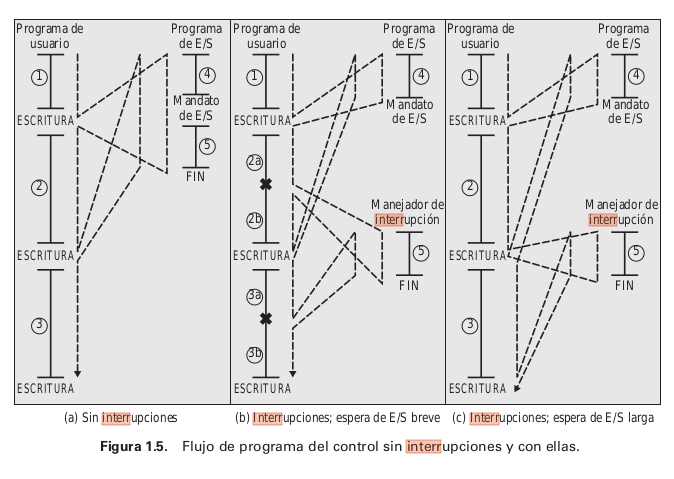
\includegraphics[scale=1,width=\textwidth]{interrupciones.png}
\end{figure}

\textbf{Eventos:excepciones e interrupciones}

Eventos o "situaciones especiales":
\begin{itemize}
\item Excepciones (síncronas): llamadas al sistema.

\item Interrupciones (asíncronas): fin de operación de DMA.
\end{itemize}

Hay otras diferencias como el origen, la predictibilidad o la reproducibilidad. El manejo de excepciones e interrupciones debe producirse a tiempo y es específico para cada tipo de procesador.

\begin{figure}[h]
\centering
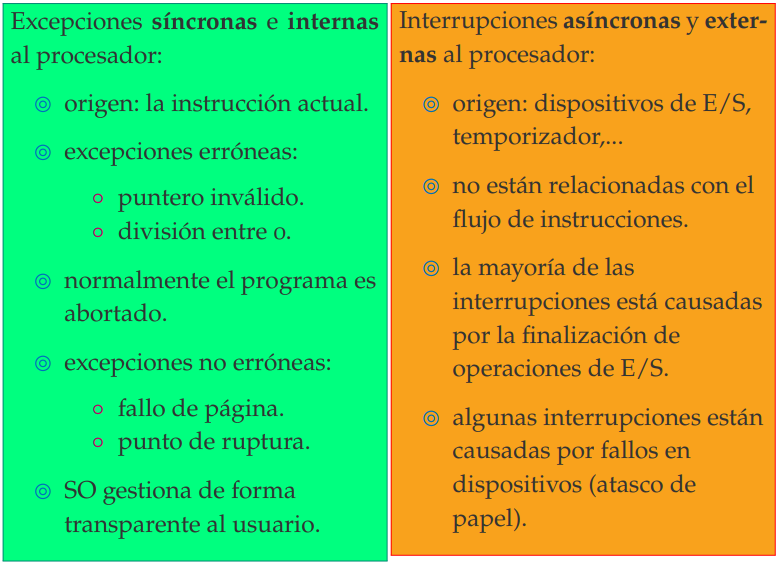
\includegraphics[scale=1,width=\textwidth]{eventos.png}
\end{figure}

\textbf{Interrupciones software (int/syscall - swi)}

Se tratan de un mecanismo para ceder el contro al SO elevando el nivel de privilegio. Son síncroncas, predecibles y reproducibles, luego aunque se llamen interrupciones son excepciones. 

Un mismo programa aislado siempre provoca las mismas:
\begin{itemize}
\item Instrucción desconocida.
\item Instrucción errónea (divisón entre 0).
\item Modo de direccionamiento erróneo.
\item Violación del espacio de direcciones.
\item Llamada al sistema.
\item Fallo de página (solo políticas de paginación locales).
\end{itemize}

Deben atenderse, sino se daría un comportamiento erróneo. Producen una sobrecarge en espacio y tiempo fuera del programa que la solicita.\\

\textbf{Interrupciones}

Se trata de un mecanismo para solicitar la atención de la CPU. Son asíncronas, no predecibles y no reproducibles. Un periférico puede solicitar una interrupción independientemente del estado de la CPU o el proceso actual.

Ejemplos:
\begin{itemize}
\item Eventos externos: sensores
\item Final de una operación DMA.
\item Final de una operación E/S.
\end{itemize}

\textbf{Vector de interrupciones}

Se trata del vector que contiene las direcciones de los manejadores de interrupción para los distintos dispositivos conectados y las distintas interrupciones.

\begin{figure}[h]
\centering
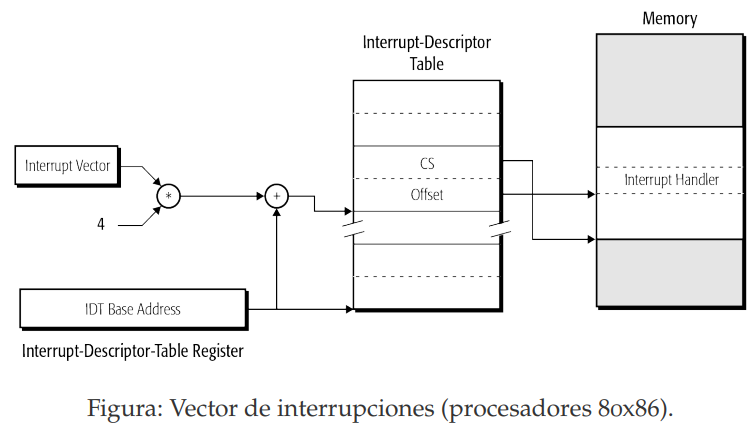
\includegraphics[scale=1,width=\textwidth]{vectorint.png}
\end{figure}

\textbf{Manejo de excepciones e interrupciones}

Los siguientes eventos podríann lanzar una excepción o una interrupción:
\begin{itemize}
\item Señales de periféricos:
	\begin{itemize}
	\item Final de una lectura de disco
	\item Atasco de papel
	\end{itemize}
	
\item Cambio del dominio de protección (segmentación/paginación).

\item Errores de programación (acceso a dirección inválida).

\item Desbordamiento de memoria (desbordamiento de pila).

\item Paginación bajo demanda.

\item Fallos hardware (paridad de memoria).
\end{itemize}

El manejo del evento se hace durante la ejecución del proceso actualmente en ejecución.\\

\textbf{Efectos de la temporización}

El manejo de cada evento ralentiza la ejecución del programa interrumpido. El resultado de los programas no se pone en peligro, salvo las aplicaciones de tiempo real que si pueden fallar. Esta es una de las razones por las que los programadores no deben confiar en las condiciones de temporización (ej: sincronización). \\

\textbf{Control de interrupciones:}

Las interrupciones pueden llegar en cualquier momento:
\begin{itemize}
\item Usuario modificando datos compartidos.

\item SO realizando una operación no interrumpible.
\end{itemize}

El sistema operativo y el hardware permiten sincronizar actividades concurrentes mediantes operaciones atómicas: secuencias de instrucciones que no pueden ser interrumpidas. \\

Soluciones:
\begin{itemize}
\item Deshabilitar las interrupciones. En una máquina monoprocesador, los procesos concurrentes no pueden solaparse, sólo pueden entrelazarse. Es más, un proceso continuará ejecutando hasta que invoque un servicio del sistema operativo o hasta que sea interrumpido. Por tanto, para garantizar la exclusión mutua, basta con impedir que un proceso sea interrumpido. Esta técnica puede proporcionarse en forma de primitivas definidas por el núcleo del sistema para deshabilitar y habilitar las interrupciones. Esta solución no funcionará sobre una arquitectura multiprocesador. Cuando el sistema de cómputo incluye más de un procesador, es posible (y típico) que se estén ejecutando al tiempo más de un proceso. En este caso, deshabilitar interrupciones no garantiza exclusión mutua.

\item Instrucciones atómicas basadas en leer/modificar/almacenar: En una configuración multiprocesador, varios procesadores comparten acceso a una memoria principal comúnt. No hay mecanismo de interrupción entre procesadores en el que pueda basarse la exclusión mutua. 

A un nivel hardware, el acceso a una posición de memoria excluye cualquier otro acceso a la misma posición. Los diseñadores de hardware han propuesto varias instrucciones que llevan a cabo dos acciones atómicamente, como leer y escribir o leer y comprobar, sobre una única posición de memoria con un único ciclo de búsqueda de instrucción. Durante la ejecución de la instrucción, el acceso a la posición de memoria se le bloquea a toda otra instrucción que referencia esa posición. Estas acciones se realizan (típicamente) en un solo ciclo de instrucción.
	\begin{itemize}
	\item \textbf{tas}: \textit{test and set} (comprueba y establece)
	
	\item \textbf{cmpxchg}: comparar e intercambiar.
	
	\item \textbf{ll/sc}: carga enlazada y almacenamiento condicional.
	\end{itemize}
\end{itemize}

La mayoría de los ordenadores permiten que los ocntroladores de E/S interrumpan la actividad del procesador. La CPU transfiere el control a un manejador de interrupción que normalmente es parte del SO (excepción: controladores en espacio de usuario).

El procesador puede prevenir las interrupciones:
\begin{itemize}
\item Enmascarándolas

\item Deshabilitándolas

\item Estableciendo un nivel mínimo de prioridad.
\end{itemize}

\textbf{Procesamiento de interrupciones}
\begin{figure}[h]
\centering
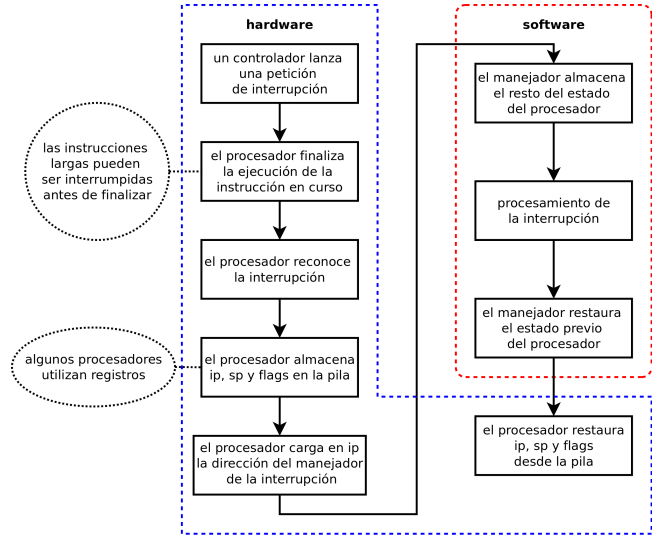
\includegraphics[scale=1,width=\textwidth]{procinterrupcion.png}
\end{figure}

\textbf{Ventajas del uso de interrupciones}
\begin{itemize}
\item Los eventos son atendidos más rápidamente

\item No se consume tiempo del procesador para descubrir el final de un evento.

\item Los programas pueden ejecutarse más rápidamente.

\item Se mejora el aprovechamiento del procesador.
\end{itemize}

Con sólo el uso de interrupciones el procesador sigue siendo el encargado de realizar las transferencias de información. La solución ideal es utilizar DMA para evitarlo.\\

\textbf{Múltiples interrupciones}
\begin{figure}[h]
\centering
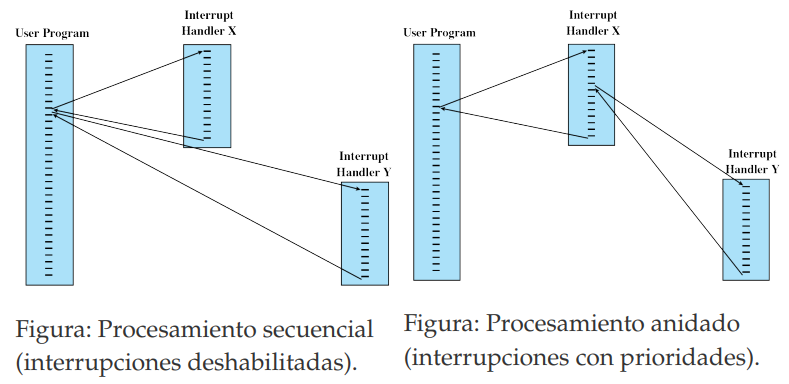
\includegraphics[scale=1,width=\textwidth]{multinterrupcion.png}
\end{figure}

\textbf{Técnicas de Entrada/Salida}
\begin{itemize}
\item \textbf{E/S programada (sondeo)}. En E/S programada, el módulo de E/S realiza la acción solicitada y fija los bits correspondiente en el registro de estado de E/S, pero no realiza ninguna acción para avisar al procesador. En concreto, no interrumpe al procesador. Por tanto, después de que se invoca la instrucción de E/S, el procesador debe tomar un papel activo para determinar cuándo se completa la instrucción de E/S. Por eso el procesador comprueba periódicamente el estado del módulo de E/S hasta que se encuentre que se ha completado la operación.

Tiene la desventaja de que es un proceso que consume un tiempo apreciable que mantiene al procesador ocupado innecesariamente.

\item \textbf{E/S dirigida mediante interrupción}. Es una alternativa a la E/S programada. En ella el procesador genera un mandato de E/S para un módulo y, acto seguido, continúa realizando algún otro trabajo útil. El módulo de E/S interrumpirá más tarde al procesador para solicitar su servicio cuando esté listo para intercambiar datos con el mismo. El procesador ejecutará la transferencia de datos, como antes, y después reanudará el procesamiento previo.

El mayor problema de esta alternativa es que el procesador tiene que hacer la transferencia de datos el mismo, cosa que se arreglará con DMA.

\item \textbf{Acceso directo a memoria (DMA)}. La función DMA puede ser llevada a cabo por un módulo separado conectado en el bus del sistema o puede estar incluida en un módulo de E/S. La técnica funciona como sigue, cuando el procesador desea leer o escribir un bloque de datos, genera un mandato de DMA, enviándo la siguiente información:
\begin{itemize}
\item Si se trata de una lectura o una escritura.

\item La dirección del dispositivo de E/S involucrado.

\item La posición inicial de memoria en la que se desea leer los datos o donde se quieren escribir.

\item El número de palabras que se pretende leer o escribir.
\end{itemize}

A continuación, el procesador continúa con otro trabajo. Ha delegado esta operación de E/S al módulo de DMA, que se ocupará de la misma. El módulo de DMA transferirá el bloque completo de datos, palabra a palabra, hacia la memoria o desde ella sin pasar a través del procesador. Por tanto, el procesador solo se involucra al principio y al final.
\end{itemize}

\begin{figure}[h]
\centering
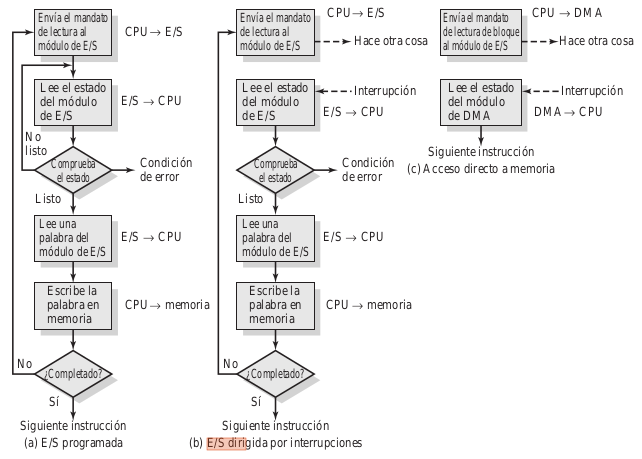
\includegraphics[scale=1,width=\textwidth]{DMA.png}
\end{figure}

\textbf{Direccionamiento físico de la memoria principal}

El direccionamiento virtual es algo que sólo existe en el interior del procesador. Para acceder a memoria los controladores de dispositivos y DMA sólo emplean direcciones físicas. Por ejemplo:
\begin{figure}[h]
\centering
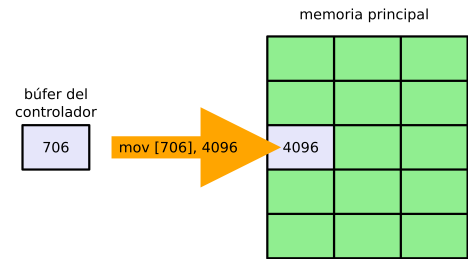
\includegraphics[scale=1,width=70mm]{ejemplo1.png}
\end{figure}

Un retraso en la E/S podría provocar que el marco 4096 fuese asignado a otro proceso a través de los mecanismos de segmentación o paginación. La solución a este problema es fijar (\textbf{pinning}) el marco de página durante el tiempo que dure el proceso de transferencia. Fijar (\textbf{pinning}) y liberar (\textbf{unpinning}) es un mecanismo de protección.
\begin{itemize}
\item Usos: soporte de DMA y procesos de tiempo real.

\item Problema: el abuso para acaparar recursos.
\end{itemize}

\begin{figure}[h]
\centering
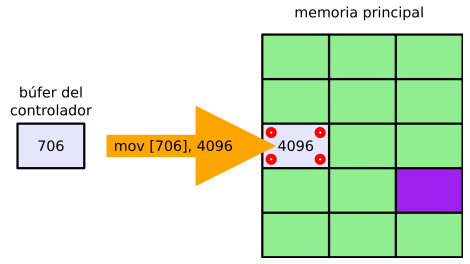
\includegraphics[scale=1,width=70mm]{pinning.png}
\end{figure}

\textbf{Temporizador}

Los niveles de privilegio son un mecanismo de protección útil para el SO. Los eventos pueden transferir el control al sistema operativo. Si un proceso no genera eventos nunca cede el control del procesador. A este problema hay varias soluciones:

\begin{itemize}
\item La más habitual: generar una interrupción de forma periódica mediante el temporizador, ej: cada 10ms.

\item La más conveniente: reprogramar el temporizador tras cada evento para que sólo genere interrupciones cuando sea necesario.
\end{itemize}

\section{Tema 2: Introducción a los sistemas operativos}
\subsection{Abstracciones}
Se denomina espacio de direcciones a la memoria utilizable por un proceso. Se trata además de una unidad de protección de memoria, pues el hardware de direccionamiento en memoria asegura que un proceso se pueda ejecutar únicamente dentro de su propio espacio de direcciones.

Habitualmente este está formado por 3 componentes:
\begin{itemize}
\item \textbf{Código:} .text

\item \textbf{Datos:} .data, .bss y heap

\item \textbf{Pila:} Stack
	\begin{itemize}
	\item Variables locales
	\item Marcos de procedimiento
	\end{itemize}
\end{itemize}

El tamaño de cada zona es:
\begin{itemize}
\item Código: tamaño fijo

\item Datos: pueden crecer hacia arriba

\item Pila: pueden crecer hacia abajo
\end{itemize}

\begin{figure}[h]
\centering
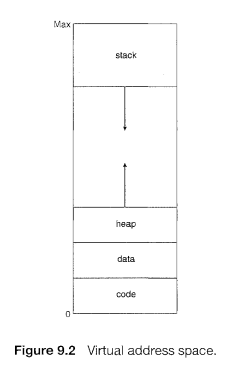
\includegraphics[scale=1, width=60mm]{adresspace.png}
\end{figure}
\newpage
\textbf{Procesos y/o hebras:}

Se trata de una unidad de trabajo. Incluye el contexto del procesador (que contiene el contador del programa y el puntero de pila) y su propia áread de datos para una pila (para posibilitar el salto a subrutinas). Un hilo se ejecuta secuencialmente y se puede interrumpir de forma que el procesador pueda dar paso a otro hilo. A parte de la distribución dada hay otras distintas como pueden ser

\begin{itemize}
\item (Porción de) un programa en ejecución.

\item Instancia de un programa ejecutándose.

\item Hebra/hilo/fibra: mínima unidad de ejecución

\item Proceso/tarea: unidad de posesión/protección de recursos.
\end{itemize}
\begin{figure}[h]
\centering
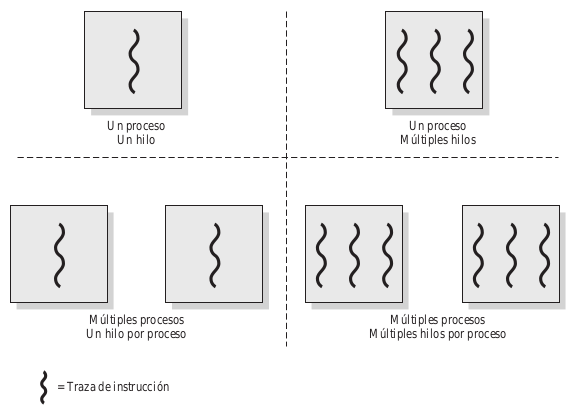
\includegraphics[scale=1, width=70mm]{hilos_programa.png}
\end{figure}

\textbf{Comunicación entre procesos}

Hay varios 3 tipos de comunicación entre procesos:

\begin{itemize}
\item Ficheros: tuberías, sockets.
	\begin{itemize}
	\item Tubería: es un \textit{buffer} circular que permite que dos procsos se comuniquen siguiendo el modelo productor consumidor. Por tanto, se trata de una cola de tipo FIFO, en la que se escribe un proceso y se lee otro.
	
	\item Socket: permite la comunicación entre un proceso cliente y un proceso servidor y puede ser orientado a conexión o no orientado a conexión. Un socket se puede considerar como un punto final en una comunicación. Un socket cliente en un computador utiliza una dirección para llamar a u socket de servidor en otro computador. Una vez que han entrado en comunicación los sockets, los dos computadores pueden intercambiar datos.
	\end{itemize}

\item Paso de mensajes. Los procesos se comunican por medio de mensajes, que son un conjunto de bytes con un tipo asociado. Asociada a cada proceso existe una cola de mensajes, que funciona como buzón.

\item Memoria compartida. Es la forma más rápida de comunicación entre procesos. Se trata de un bloque de  memoria virtual compartido por múltiples procesos. Los procesos leen y escriben en la memoria compartida utilizan las mismas instrucciones de máquina que se utilizan para leer y escribir en otras partes de su espacio de memoria virutal.
\end{itemize}

En algunos libros no se considera la tubería como un tipo de comunicación en sí mismo, ya que quería dentro de alguno de los otros dos.

\begin{figure}[h]
\centering
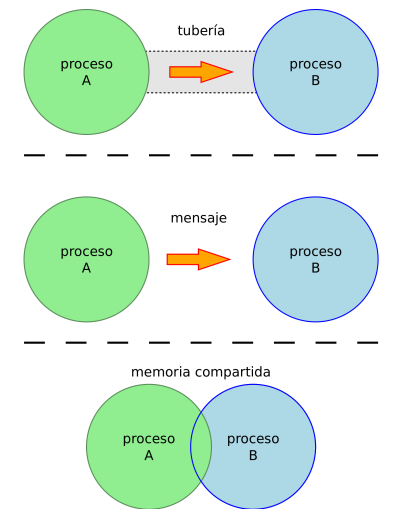
\includegraphics[scale=1, width=60mm]{tipos_com.png}
\end{figure}

\textbf{Concurrencia y paralelismo:}

Varios procesos pueden ejecutarse,
\begin{itemize}
\item en paralelo en un multiprocesador.

\item de forma concurrente en un uniprocesador.
\end{itemize}

No se debe confundir concurrencia con paralelismo, pues aunque la concurrencia da una impresión de paralelismo, realmente lo único que hace es un empleo muy eficiente del tiempo de ejecución del procesador, dando lugar a la sensación de ejecución de varios procesos simultáneamente, pero relamente en ningún momento el procesador tiene en ejecución dos procesos distintos en el mismo instante.

\begin{figure}[h]
\centering
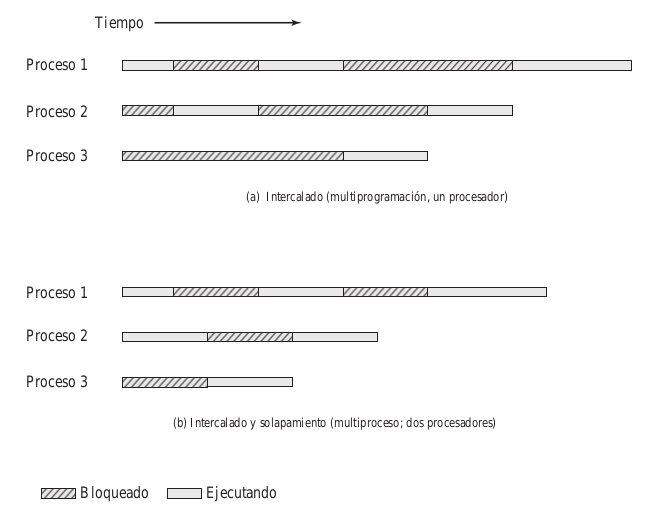
\includegraphics[scale=1, width=\textwidth]{concurrenciavsparalelismo.png}
\end{figure}

Los procesos multihebra pueden ser ejecutados de forma paralela o concurrente en función de
\begin{itemize}
\item el número de procesadores

\item el modelo de hebras: usuario o núcleo.
\end{itemize}

Podrán aparecer "condiciones de carrera" si no manejamos cuidadosamente la concurrencia, lo que implica la necesidad de métodos de sincronización de procesos y hebras.

\textbf{Condiciones de carrera:} sucede cuando múltipres procesos o hilos leen y escriben datos de forma que el resultado final depende del orden de ejeucicón de las instrucciones en los múltiples procesos.\\

\textbf{Gestión de memoria.}

La memoria RAM es limitada. De aquí surge el problema de que los procesos no saben qué posición ocuparán en la RAM. La posición de los procesos en RAM es responsabilidad del compilador y del sistema operativo. La solución a este problema es la utilización de código relocalizable. Este código tiene la particularidad de que en vez de trabajar con direcciones físicas trabaja con direcciones relativas al código, es decir, en lugar de hacer un salto a la dirección 0xffff, se hace un salto a la dirección en la que está la instrucción actual-5. De esta forma ya no es necesario saber exactamente donde está cada cosa, sino que se buscará donde está la ejecución instrucción actual-5, cuya dirección puede variar entre ejecuciones (o incluso dentro de la misma ejecución). 

Otro problema que surge es que la necesidad de memoria de todos los procesos activos pueden ser mayores que la RAM. La solución es el uso de memoria virtual, la cual da al proceso la impresión de tener más memoria disponible de la que realmente tiene, y este diferencia entre la memoria real y la virtual se suple con la carga de páginas de memoria bajo demanda. De esta forma no se requiere que todo el proceso esté cargado en memoria, sino unas ciertas páginas concretas, y se cargan las que se necesitan según la demanda del programa.\\

\textbf{Memoria virtual:} Permite al programador direccionar memoria de forma razonable en cuanto a

\begin{itemize}
\item Cantidad: los procesoso creen disponer de toda la RAM.

\item Seguridad: los espacios de direcciones son independientes. Una misma dirección virtual en dos espacios de direcciones distintos puede ser mapeada en diferentes posiciones en la RAM.

\item El mapeado de porciones de memoria virtual en memoria física se hace de forma automática, liberando así al programador de esta tarea.
\end{itemize}

El funcionamiento eficiente de la memoria virtual requiere soporte hardware.\\

Con la memoria virtual las aplicaciones creen tener un espacio de direcciones plano. La memoria física se divide en prociones. Las regiones no necesitan mapearse de forma continua, a excepción de la E/S mapeada en memoria (controladores). (Para maś información ver la explicación de memoria virtual del tema 1).

\begin{figure}[h]
\centering
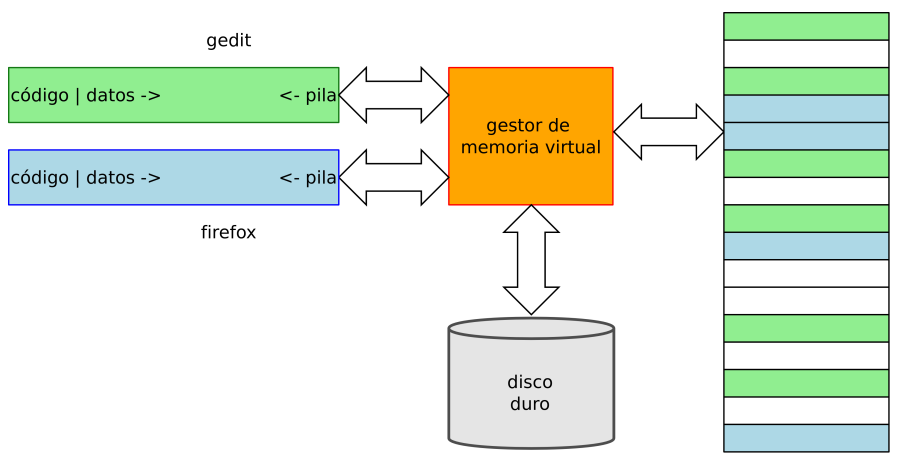
\includegraphics[scale=1, width=\textwidth]{mem_virtual.png}
\end{figure}

\textbf{Planificación/gestión de recursos}

\begin{itemize}
\item Equidad: normalmente, se desea que todos los procesos que compiten por un determinado recurso, se les conceda un acceso equitativo a dicho recurso. Esto es especialmente cierto para trabajos de la misma categoría, es decir, trabajos con demandas similares.

\item Tiempo de respuesta: el sistema operativo puede necesitar discriminar entre diferentes clases de trabajos con diferentes requisitos de servicio. El sistema operativo debe tomar las decisiones de asignación y planificación con el objetivo de satisfacer el conjunto total de requisitos. Además, debe tomar las decisiones de forma dinámica. 

\item Eficiencia: el sistema operativo debe intentar maximizar la proximidad, minimizar el tiempo de respuesta, y, en caso de sistemas de tiempo compartido, acomodar tantos usuarios como sea posible. Estos criterios entran en conflicto: encontrar un compromiso adecuado en una situación particular es un problema objeto de la investigación sobre sistemas operativos.
\end{itemize}

Diferencia entre políticas y mecanismos:
\begin{itemize}
\item Planificación $\Leftrightarrow$ apropiación/explusión

\item Paginación $\Leftrightarrow$ reemplazo.

\item Interacción $\Leftrightarrow$ comunicación.
\end{itemize}

\textbf{Gestión de E/S:}

Clasificación de dispositivos de E/S:
\begin{itemize}
\item Dispositivos de caracteres: aquellos que envían o reciben un flujo de carateres, sin sujetarse a una estructura de bloques. No se pueden utilizar direcciones ni tienen una operación de búsqueda. Ejemplos: puerto de serie, módem, ratón, ...

\item Dispositivos de bloques: aquellos que almacenan la información en bloques de tamaño fijo, cada uno con su propia dirección. Ejemplos: discos duros, tarjetas de red, ...
\end{itemize}

Papel de la gestión de dispositivos $\Rightarrow$ interfaz:
\begin{itemize}
\item Porporcionar una interfaz genérica, como en UNIX. En UNIX cada dispositivo de E/S está asociado con un fichero especial, que lo gestiona el sistema de ficheros y se lee y escribe de la misma manera que los ficheros de datos de usuario. Esto proporciona una interfaz bien definida y uniforme para los usuarios y los procesos. Para leer o escribir de un dispositivo, se realizan peticiones de lectura o escritura en el fichero especial asociado con el dispositivo.

\item Proporcionar una interfaz específica para cada tipo de dispositivo, como en Windows. Windows dispone de un gestor de E/S, que es responsable de todo el sistema de E/S del sistema operativo y proporciona una interfaz uniforme a la que todos los tipos de manejadores pueden llamar. 
\end{itemize}

\begin{figure}[h]
\centering
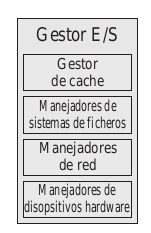
\includegraphics[scale=1,width=50mm]{ES_windows.png}
\end{figure}

Componentes de un controlador de dispositivo (software):
\begin{itemize}
\item Código de inicialización

\item Llamada al sistema para responder a las peticiones de usuario

\item Manejador de interrupción para responder a las peticiones del controlador de dispositivo (hardware)
\end{itemize}

\textbf{Ficheros}

Implementación del almacenamiento persistente o a largo plazo. Las unidades almacenadas persistentemente son objetos como:
\begin{itemize}
\item Ficheros

\item Directorios
\end{itemize}

Tipos de ficheros:
\begin{itemize}
\item Tradicionales: gestionados a través de llamadas al sistema.

\item Mapeados en memoria: se gestionan igual pero se almacenan en la memoria principal.
\end{itemize}

\textbf{Interacción de los componentes del sistema}

\begin{figure}[h]
\centering
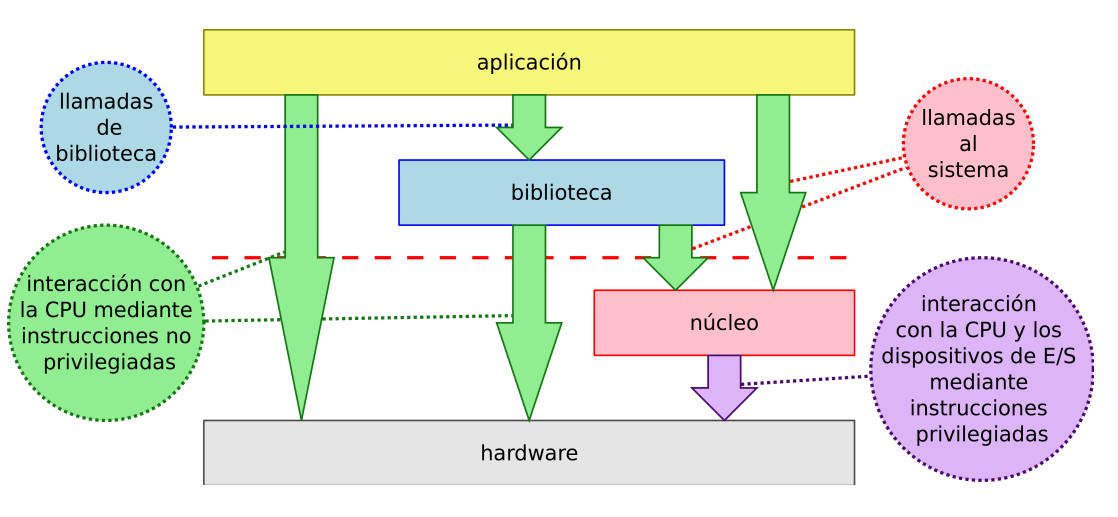
\includegraphics[scale=1, width=\textwidth]{interaccion_sistema.png}
\end{figure}

\textbf{Interfaz de programación de aplicaciones (API)}

Existen dos interfaces de programación para acceder a los servicios proporcionados por el núcleo del SO:
\begin{itemize}
\item Llamadas al sistema: interfaz directa con el núcleo.

\item API: interfaz indirecta escrita en algún lenguaje de alto nivel (funciones de biblioteca).
\end{itemize}

Las 3 APIs más conocidas son:
\begin{itemize}
\item Win32/Win64

\item POSIX: Portable Operating System Interface (UNIX)

\item Java
\end{itemize}

\textbf{Paso de parámetros:}

A menudo es necesaria más informació que la identificación de la llamada al sistema. El tipo y cantidad de información varia entre llamadas.

Métodos de paso de parámetros:
\begin{itemize}
\item Registros: método rápido pero de poca capacidad

\item Memoria: la aplicación agrupa los parámetros en un área de memoria y pasa la localización de dicha área mediante un registro.

\item Pila: los parámetros son apilados por la aplicación y desapilados por la llamada al sistema.
\end{itemize}

El empleo de memoria tiene la ventaja de no limitar el número ni el tamaño de los parámetros, pero es más lenta que los registros (velocidad+copia). La estrategia más flexible para el paso de parámetros es la pila.

\subsection{Llamadas al sistema}
\begin{itemize}
\item \textbf{Gestión de procesos}

\begin{figure}[h]
\centering
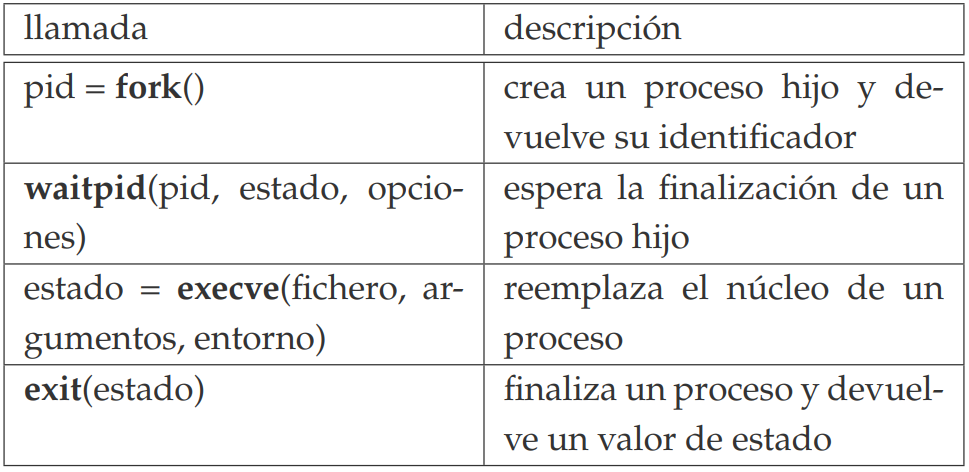
\includegraphics[scale=1, width=\textwidth]{llamadas_1.png}
\end{figure}
\newpage

\item \textbf{Gestión de ficheros:}

\begin{figure}[h]
\centering
\includegraphics[scale=1, width=110mm]{llamadas_2.png}
\end{figure}

\item \textbf{Gestión de directorios}
\begin{figure}[h]
\centering
\includegraphics[scale=1, width=110mm]{llamadas_3.png}
\end{figure}
\newpage

\item \textbf{Otras llamadas al sistema}
\begin{figure}[h]
\centering
\includegraphics[scale=1, width=110mm]{llamadas_4.png}
\end{figure}

\item \textbf{Comparativa POSIX/Win32}
\begin{figure}[h]
\centering
\includegraphics[scale=1, width=110mm]{comparativa.png}
\end{figure}

\end{itemize}

\section{Tema 3: Historia de los Sistemas Operativos}
\subsection{Definición}
\textbf{Sistema operativo:} programa o conjunto de programas encargado de gestionar los recursos de la máquina y proveer servicios al resto de programas. Suele ejecutarse en modo privilegiado. Controla la ejecución de aplicaciones y programas y actúa como interfaz entre las aplicaciones y el hardware del computador. 

Suelen venir junto con multitud de otros programas, que sin forma parte del sistema operativo, resultan de suma utilidad: intérprete de órdenes, editor de texto, gestor de ficheros, navegador, ...

\subsection{Historia}
\subsubsection{Primera generación (1945-1955): Tubos de vacío y paneles}
En esta primera generación los sistemas operativos servían como máquinas de cálculo. Se trataban de dispositivos mecánicos que utilizaban tubos de vacío y paneles.

Para programas estos se utilizaban cables, interruptores y tarjetas perfoardas. Un gran problema de estos era que el diseño, construcción, operación, programación y mantenimiento requería de genios como Aiken, von Neuman o Mauchley.

\subsubsection{Segunda generación (1955-1965): Transistores y sistemas por lotes}
En esta segunda generación los siststamas operativos se utilizaban para el cálculo científico y la ingeniería. La invención del transistor permitió que se redujera el tamaño y precio de estos y los popularizó dando lugar a mainframes como el IBM 1401 o el IBM 7094.

Para programas estos se utilizaba lenguaje ensamblador y lenguajes se alto nivel (FORTRAN) sobre tarjetas perforadas. Por otro lado, se pasó del procesamiento secuencial al procesamiento por lotes. Ejemplos: FMS y IBSYS.

\begin{figure}[h]
\centering
\includegraphics[scale=1, width=\textwidth]{solotes.png}
\end{figure}

\subsubsection{Tercera generación (1965-1980): Circuitos integrados y multiprogramación}
En esta tercera generación a parte de seguir utilizandose los computadores para el cálculo científico y la ingeniería se utilizan para el procesamiento de caracteres. 

Se comienzan a utilizar ciercuitos integrados que son más baratos y se convierten en más populares (IBM 360, GE-645, DEC PDP-1).

Como logro más destacables tenemos:
\begin{itemize}
\item Multiprogramación.

\item Spooling.

\item Tiempo compartido.
\end{itemize}

Ejemplos: OS/360, CTSS, MULTICS, UNIX.

\begin{figure}[h]
\centering
\includegraphics[scale=1, width=100mm]{multiprogramacion.png}
\end{figure}

\subsubsection{Cuarta generación (1980-hoy): Ordenador personal (era $\mu$)}
La empresa (V)LSI de circuitos integrados proporciona circuitos más baratos y por consiguiente se convirtieron en más populares, dando lugar a computadores como el IBM PC.

Surgen arquitecturas de procesadores como los 8080, Z80, 80x86, Alpha, Ultrasparc, ARM.\\

Como logros destacables tenemos:
\begin{itemize}
\item GUI (Graphic User Interface).

\item SO de red. Sistema operativo especializado para dispositivos de red como pueden ser un router o un switch.

\item SMP (Symmetric Multi-Processing).

\item SO distribuidos.
\end{itemize}

Ejemplos: UINX, CP/M, MS-DOS, Linux, MacOS, Windows.\\


\subsection{Estructura}
\textbf{Clasificación:}
\begin{itemize}
\item Estructura simple:
	\begin{itemize}
	\item Monolíticos. Son sistemas operativos en los cual el núcleo proporciona la mayoría de las funcionalidades propias del sistemas operativo, incluyendo la planificación, los sistemas de ficheros, las redes y otras funciones.
	
	\item Capas. Las funciones se organizan jerárquicamente y sólo hay interacción entre las capas adyacentes. Con el enfoque por capas, la mayor parte o todas las capas ejecutan en modo núcleo.
	
	\item Modulares
	\end{itemize}

\item Estructura cliente/servidor:
	\begin{itemize}
	\item Micronúcleo. Asigna unas pocas funciones esenciales al núcleo, incluyendo los espacios de almacenamiento, comunicación entre procesos y planificación básica.
	
	\item Exonúcleo.
	\end{itemize}
	
\item Máquina virtual.

\item Híbridos
\end{itemize}

\textbf{Tendencias:}
\begin{itemize}
\item Núcleos Extensibles

\item Multiservidores sobre un micronúcleo.

\item Núcleos híbridos.
\end{itemize}

\textbf{Monolítico:}

El Sistema operativo completos se ejecuta en modo protegido. Como consecuencia hay una protección nula entre los componentes del mismo, pues cualquier fallo puede afectar a cualquier parte del sistema operativo.\\

Ventajas:
\begin{itemize}
\item Es muy eficiente gracias a la economía de cambios de contexto. Esto se debe a que gracias a que todo el SO se ejecuta en modo protegido no requiere de cambios de contexto mientras se ejecutan llamadas al sistema.
\end{itemize}

Desventajas:
\begin{itemize}
\item La falta de protección implica una menor fiabilidad. 

\item Mal manejo de la complejidad. Es más sentillo escribir 1000 programas de 1000 líneas que uno de 1000000
\end{itemize}

\begin{figure}[h]
\centering
\includegraphics[scale=1, width=90mm]{monolitico.png}
\end{figure}

\textbf{Capas/Niveles:}

El Sistema Operativo completo se ejecuta en modo protegido. Hay una escasa división entre los componentes.\\

Ventajas:
\begin{itemize}
\item Es muy eficiente gracias a la economía de cambios de contexto.

\item La complejidad es menor que la de los sistemas operativos monolíticos.
\end{itemize}

Desventajas:
\begin{itemize}
\item La falta de protección implica una menor fiabilidad.

\item Menos flexible que un sistema operativo monolítico.

\item Es difícil subdividir adecuadamente las capas.
\end{itemize}

\begin{figure}[h]
\centering
\includegraphics[scale=1,width=90mm]{capasniveles.png}
\end{figure}

\textbf{Modular:}

El Sistema Operativo se ejecuta en modo protegido. Una vez más esto implica una escasa protección entre los componentes.\\

Ventajas:
\begin{itemize}
\item De nuevo la econocomías de cambios de contexto lo hace eficiente.

\item Tiene una menos complejidad.
\end{itemize}

Desventajas:
\begin{itemize}
\item La falta de protección implica una menor fiabilidad.

\item Es menos flexible que un sistema operativo monolítico.

\item Es difícil elegir que colocar en el núcleo y que en los módulos.
\end{itemize}

\begin{figure}[h]
\centering
\includegraphics[scale=1, width=90mm]{modular.png}
\end{figure}
\newpage

\textbf{Micronúcleo/Microkernel}

Una mínima parte del Sistema Operativo se ejecuta en modo protegido. \\

Ventajas:
\begin{itemize}
\item La perfecta protección entre componente nos da una mayor fiabilidad

\item Manejo de la complejidad.

\item Facilidad de programación
\end{itemize}

Desventajas:
\begin{itemize}
\item Debido a la sobrecarga en las comunicaciones hay una menor eficiencia.
\end{itemize}

\begin{figure}[h]
\centering
\includegraphics[scale=1,width=90mm]{microkernel.png}
\end{figure}

\newpage

\textbf{Exonúcleo:}

Apenas existe el sistema operativo, sólo un gestor de recursos. En este tipo de sistema operativo dejamos que el software accedad directamente al hardware.\\

Ventajas:
\begin{itemize}
\item Perfecta protección entre componentes, lo cual da lugar a una alta fiabilidad.

\item El acceso directo al hardware nos dá lugar a una máxima eficiencia.
\end{itemize}

Desventajas:
\begin{itemize}
\item Pobre reutilización del código.
\end{itemize}

\begin{figure}[h]
\centering
\includegraphics[scale=1, width=90mm]{exonucleo.png}
\end{figure}

\newpage

\textbf{Máquina virtual:}

Se trata de copias virtuales de la máquina rela:
\begin{itemize}
\item SW: Bochs, Qemu, VMWare, Xen.

\item HW: VMWare, Xen
\end{itemize}

Ventajas:
\begin{itemize}
\item Perfecta protección entre componentes, lo que garantiza una alta fiabilidad.

\item Mejor aprovechamiento del hardware.

\item Máxima reutilización del código.
\end{itemize}

Desventajas:
\begin{itemize}
\item La simulación del hardware real puede ser costosa, dando lugar a una baja eficiencia.
\end{itemize}

Esta opción es un éxito gracias a mejoras en el HW.

\begin{figure}[h]
\centering
\includegraphics[scale=1, width=90mm]{maquinavirtual.png}
\end{figure}

\newpage
\textbf{Híbrida}

\begin{itemize}
\item La mezcla más frecuente es la combinación de micronúcleo y monolítico.

\item Ventaja: ganamos velocidad respecto al micronúcleo.

\item Desventaja: perdemos protección entre componentes.
\end{itemize}

\begin{figure}[h]
\centering
\includegraphics[scale=1,width=90mm]{hibrida.png}
\end{figure}

\newpage
\subsection{Ejemplos}
\textbf{MS-DOS}
\begin{figure}[h]
\centering
\includegraphics[scale=1,width=\textwidth]{MSDOS.png}
\end{figure}

\newpage

\textbf{Windows 2000}
\begin{figure}[h]
\centering
\includegraphics[scale=1,width=\textwidth]{WINDOWS2000.png}
\end{figure}

\newpage

\textbf{Linux}
\begin{figure}[h]
\centering
\includegraphics[scale=1,width=\textwidth]{linux.png}
\end{figure}

\newpage

\textbf{Mach}
\begin{figure}[h]
\centering
\includegraphics[scale=1,width=\textwidth]{mach.png}
\end{figure}

\textbf{MacOS X}
\begin{figure}[h]
\centering
\includegraphics[scale=1, width=105mm]{MacOSX.png}
\end{figure}

\newpage

\textbf{QNX}
\begin{figure}[h]
\centering
\includegraphics[scale=1,width=\textwidth]{qnx.png}
\end{figure}

\newpage
\subsection{Comparativa}
\subsubsection{Coste estructural de una llamada al sistema: caso monolítico}
\textbf{1 llamada al sistema:}
\begin{enumerate}
\item Entrada al núcleo.

\item Cambio al espacio de direccionies del núcleo.

\item Salida del núcleo.
\end{enumerate}

\textbf{1 llamada a procedimiento:} llamada y retorno en el interior del espacio de direcciones del núcleo y pudiendo compartir información.

\begin{figure}[h]
\centering
\includegraphics[scale=1,width=100mm]{llamada_sistema.png}
\end{figure}
\newpage

\subsubsection{Coste estructural de una llamada al sistema: caso micronúcleo}
\textbf{4 llamadas al sistema:}
\begin{enumerate}
\item Entrada al micronúcleo.

\item Cambio al espacio de direcciones del micronúcleo.

\item Transferencia del mensaje.

\item Recuperar el espacio de direcciones original.

\item Salida del micronúcleo.
\end{enumerate}

\begin{figure}[h]
\centering
\includegraphics[scale=1,width=\textwidth]{llamada_kernel.png}
\end{figure}

\newpage

\subsubsection{Coste estructural: multiservidor}
\begin{figure}[h]
\centering
\includegraphics[scale=1, width=\textwidth]{multisevidor.png}
\end{figure}





\end{document}
